\newcommand{\LF}{\text{LF}}

\section{抗泄漏安全}
%写作思路: 先参考Kalai和Reyzin的综述~\cite{KR-ePrint-2019}先给出一段关于抗泄漏PKE的综述, 
%然后聚焦bounded leakage model, 先介绍~\cite{NS-CRYPTO-2009}, 再介绍你的ASIACRYPT、PKC和我的ASIACRYPT合并起来. 
%可选的: 介绍一下randomness leakage resilience, 方案就是我们以前讨论过的HPS对偶方案.  

侧信道攻击, 又称边信道攻击或旁路攻击,利用密码算法在实现过程中泄漏的物理信息, 如运行时间~\cite{Kocher-CRYPTO-1996}、电磁辐射~\cite{GMO-CHES-2001}、能量功耗~\cite{Kocher-CRYPTO-1999}等来攻击密码算法的安全性. 图~\ref{fig:ch5-SCA}展示了侧信道攻击的方法, 其中, $\text{F}$代表一种密码算法函数, 如签名算法、解密算法等. 除了私钥$sk$外, 算法的输入可能还包括签名消息或解密密文$x$. 敌手可以利用上述侧信道攻击方法在算法$\text{F}$执行过程中获取私钥$sk$的部分信息, 记作$\mathsf{leak}(sk)$. 2008年, Halderman等人~\cite{Halderman-USENIX-Security-2008}还发现另一类特殊的侧信道攻击方法, 即``冷启动''攻击(又称内存攻击). 简单来说, 计算机断电后内存中存储的信息并不是立即被擦除掉, 通过短暂的物理访问可以恢复动态随机存取存储器中的数据或密钥. 上述这些物理信息都有可能泄漏密钥的部分信息, 因此这类侧信道攻击统称为密钥泄漏攻击. 与传统的数学分析方法相比, 这类新型分析技术更有效, 对密码算法的安全性构成巨大的威胁. 早期抵御侧信道攻击的方法主要通过在算法实现过程中引入一些随机信息以减少泄漏的物理信息中含有的密钥信息, 可参考文献~\cite{EHCC-Book-2005}第29章及其引文. 然而这种方式难以同时抵抗多种类型的侧信道攻击技术并且这些方法缺少严格的安全性证明. 类似不可区分选择密文攻击模型, 如何建立合理的抗密钥泄漏攻击的安全模型, 并从算法角度设计可证明安全的抗密钥泄漏密码方案是抗泄漏密码学研究的主要问题.

\begin{figure}[htp!]
\begin{center}
\begin{tikzpicture}
    \node [name=Func, shapenode, thick] {$\mathsf{F}$~~~\red{$sk$}~~~~~};  
    \node [name=input, textnode,  above of=Func, xshift=0em, yshift=3em] {$x$}; 
    \node [name=output, textnode, below of=Func, xshift=0em, yshift=-3em] {$\mathsf{F}(sk, x)$}; 
    \draw (input) edge[->] (Func);
    \draw (Func) edge[->] (output);

    \node [name=adversary, left of = Func, xshift=-9em] {
\includegraphics[width=0.5in]{figure/adversary.png}};

    \node [name=radiation, textnode, left of=Func, xshift=-8em, yshift=5em] 
        {
\includegraphics[width=0.3in]{figure/attacks/radiation.png}};
    \draw (radiation) edge[color=red, thin, ->, decorate, 
        decoration={snake,amplitude=.4mm,segment length=1mm,pre length=1mm, post length=1mm}] ($(Func.west)+(0em, 0.5em)$);

    \node [name=power, textnode, left of=Func, xshift=-8em, yshift=1.5em] 
        {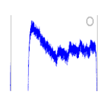
\includegraphics[width=0.3in]{figure/attacks/power.png}};
    \draw (power) edge[color=red, thin, ->, decorate, 
        decoration={snake,amplitude=.4mm,segment length=1mm,pre length=1mm, post length=1mm}] ($(Func.west)+(0em, 0.2em)$);

    \node [name=timing, textnode, left of=Func, xshift=-8em, yshift=-1.5em] 
         {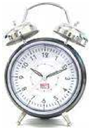
\includegraphics[width=0.3in]{figure/attacks/timing.png}};
    \draw (timing) edge[color=red, thin, ->, decorate,  
        decoration={snake,amplitude=.4mm,segment length=1mm,pre length=1mm, post length=1mm}] ($(Func.west)+(0em, -0.2em)$);

    \node [name=sound, textnode, left of=Func, xshift=-8em, yshift=-5.5em] 
         {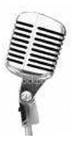
\includegraphics[width=0.25in]{figure/attacks/sound.png}};
    \draw (sound) edge[color=red, thin, ->, decorate,  
        decoration={snake,amplitude=.4mm,segment length=1mm,pre length=1mm, post length=1mm}] ($(Func.west)+(0em, -0.5em)$);

      \node [name=leak, textnode, right of = Func, xshift=12em] {$\mathsf{leak}(sk)$};  
    \draw (Func) edge[color=blue, ->, decorate, 
      decoration={snake,amplitude=.4mm,segment length=1mm,pre length=1mm, post length=1mm}] 
      node [above,yshift=1em] {
\includegraphics[width=0.8in]{figure/attacks/openssl-heartbleed.png}} 
      node [below,yshift=-1em] {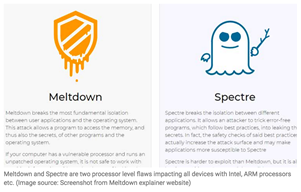
\includegraphics[width=0.8in]{figure/attacks/meltdown.png}} 
      (leak);
\end{tikzpicture}
\end{center}
\caption{侧信道攻击方法示意图}\label{fig:ch5-SCA}
\end{figure}

根据泄漏函数的形式不同, 密钥泄漏模型可以分为有界密钥泄漏和无界密钥泄漏. 2009年, Akavia、Goldwasser和Vaikuntanathan~\cite{AGV-TCC-2009}受``冷启动''攻击的启发, 提出一种非常实用的刻画密钥泄漏的模型. 该模型允许攻击者获得密钥的任意信息, 只要所有获取的信息比特长度不超过某一阈值$\lambda$即可. 因此, 该模型一般称为有界密钥泄漏模型(Bounded-Leakage Model, 简称BLM模型). 具体来讲, 攻击者可以通过一系列有效、可计算函数$f$, 称之为泄漏函数, 适应性地访问私钥$sk$, 并获取相应的泄漏信息$f(sk)$, 而对攻击者的要求是所有泄漏函数的输出长度之和不超过该阈值. 由于BLM模型既简单又能涵盖广泛的侧信道攻击方法, 近年来, 该模型得到了密码学界的广泛关注. 特别地, 有界密钥泄漏模型可以涵盖以下两种密钥泄漏情形: 相对泄漏(Relative Leakage)和绝对泄漏(Absolute Leakage).
\begin{itemize}
\item\textbf{相对泄漏:} 指总体泄漏量与私钥长度的比率是相对固定的. 这一比率通常称为相对泄漏比率. 例如, 攻击者得到的泄漏信息长度不超过私钥长度的一半. 相对泄漏能够刻画多种侧信道攻击的情景, 包括Halderman等人的``冷启动''攻击、针对智能卡的微波攻击等. 因此, 很多抗密钥泄漏方案都是在相对泄漏模型下设计的.
\item\textbf{绝对泄漏:} 指相对泄漏量可以非常巨大. 这种模型在一些场合是非常实用的. 例如, 当系统中存有恶意软件时, 病毒程序可能会将用户大量的敏感数据传送给远程的控制服务器. 但是在很多情况下, 病毒程序下载巨量数据消耗的时间和代价很大. 因此, 抵御这种类型侧信道攻击最好的方法是将私钥变得巨大, 以至于攻击者无法获取超过阈值的信息量. Crescenzo等人~\cite{CLW-TCC-2006}和Dziembowski~\cite{Stefan-TCC-2006}将这一模型称为有界恢复模型(Bounded Retrieval Model, 简称BRM模型). 在有界恢复模型中, 设计密码算法的基本方式是通过增加敏感数据的存储空间来实现安全性, 但是不能影响系统其他方面的性能. 特别地, 合法用户仅需要访问很小一部分的密钥信息, 而他的计算和通信开销并不会有太大的增加.
\end{itemize}

有界恢复模型可以看做是内存泄漏模型的推广. 在BRM模型中设计方案的困难性主要在于方案效率仅能依赖方案的安全参数, 而不能依赖私钥的大小. 在相对泄漏模型中, 方案的效率一般与私钥大小有关. 通过扩大私钥空间来提高私钥泄漏量的同时, 方案的效率往往会显著下降. 尽管如此, 在BRM模型中设计方案通常先在相对泄漏模型中进行设计. 为此, 本节重点介绍相对泄漏模型下的抗泄漏公钥加密方案的几种典型设计方法.

\subsection{安全模型}
本节主要介绍公钥加密方案的有界密钥泄漏安全模型$\lambda$-BKL-CCA安全模型. 在该模型中, 敌手不仅可以访问解密谕言机, 而且可以获得密钥的部分信息. 密钥泄漏查询由任意一组输出长度之和不超过泄漏上界$\lambda$的函数组成. 敌手可以适应性地选择函数$f$并获得密钥的函数值$f(sk)$. 很显然, 如果函数$f$的输出没有任何限制, 则任何(公钥)加密方案都不可能抵抗密钥泄漏攻击.
\begin{trivlist}
\item \textbf{BKL-CCA安全性.} 定义公钥加密方案敌手$\mathcal{A} = (\mathcal{A}_1, \mathcal{A}_2)$的优势函数如下: 
\begin{displaymath}
	\AdvA(\kappa) = \Pr\left| \left[ \beta' = \beta:~
	\begin{array}{ll}
		& pp \leftarrow \mathsf{Setup}(1^\kappa); \\		
		& (pk, sk) \leftarrow \mathsf{KeyGen}(pp);\\
		& (m_0, m_1, state) \leftarrow \mathcal{A}_1^{\blue{\Odecrypt(\cdot)},\blue{\Oleak}}(pp, pk); \\
		& \beta \sample \{0,1\};\\ 
        & c^* \leftarrow \mathsf{Encrypt}(pk, m_\beta);\\
        & \beta' \leftarrow \mathcal{A}_2^{\blue{\Odecrypt(\cdot)}}(pp, pk, state, c^*);
	\end{array} 
\right] - \frac{1}{2}\right|,
\end{displaymath}
在上述定义中, $\mathcal{A} = (\mathcal{A}_1, \mathcal{A}_2)$的含义类似IND-CCA安全模型中的敌手, 表示敌手$\mathcal{A}$可划分为两个阶段, 划分界线是接收到挑战密文$c^*$前后, $state$表示$\mathcal{A}_1$向$\mathcal{A}_2$传递的信息, 记录部分攻击进展. $\Odecrypt(\cdot)$表示解密谕言机, 其在接收到密文$c$的询问后输出$\mathsf{Decrypt}(sk, c)$. $\Oleak$表示密钥泄漏谕言机, 其在接收到泄漏函数$f_i: \{0, 1\}^*\rightarrow\{0, 1\}^{\lambda_i}$的询问后输出$f_i(sk)$且所有泄漏函数输出长度之和满足$\sum_i\lambda_i\leq \lambda$. 如果任意的PPT敌手$\mathcal{A}$在上述游戏中的优势函数均为可忽略函数, 则称公钥加密方案是$\lambda$-BKL-CCA安全的.  
\end{trivlist}

\begin{note}
在BKL-CCA模型中, 敌手在获得挑战密文后是不允许再访问密钥泄漏服务的. 否则, 敌手可以通过编辑挑战密文的解密函数来获得明文的部分比特信息, 从而区分挑战密文加密的是$m_0$还是$m_1$. 不可区分或语义安全性的要求是非常高的, 它不允许敌手获得任何除消息空间分布之外的有用信息. 如果允许敌手在看到挑战密文后继续访问密钥泄漏函数, 则模型的安全目标必然会降低. 为此, 2011年Halevi和Lin~\cite{HL-TCC-2011}提出"After-the-fact"密钥泄漏模型, 利用明文的剩余熵来刻画方案的安全性. 在上述定义中, 若不允许敌手访问任何解密服务, 则这就是$\lambda$-BKL-CPA安全模型的定义; 若令$\lambda=0$, 即敌手没有访问密钥泄漏谕言机, 则上述定义即是标准IND-CCA安全性的定义.        
\end{note}

\subsection{NS09方案}
\subsubsection{基于哈希证明系统的通用构造}
2009年, Naor和Segev~\cite{NS-CRYPTO-2009}基于哈希证明系统提出一种抗泄漏公钥加密方案的通用构造方法. 该方案结构简单, 是哈希证明系统在抗泄漏密码学中的一个经典应用案例.

\begin{construction}[Nao-Segev BKL-CPA方案]
令$\lambda = \lambda(\kappa)$为密钥泄漏量的上界, $\epsilon_1$和$\epsilon_2$是两个可忽略的量. 该方案依赖一个$\epsilon_1$-universal哈希证明系统$\text{HPS} = (\text{HPS}.\mathsf{Setup}, \text{HPS}.\mathsf{KeyGen} \text{HPS}.\mathsf{PubEval}, \text{HPS}.\mathsf{PrivEval})$和一个平均情况下$(\log\Pi-\lambda, \epsilon_2)$-强提取器$\mathsf{Ext}: \Pi\times\{0, 1\}^t\rightarrow\{0, 1\}^m$.
\begin{itemize}
\item $\mathsf{Setup}(1^\kappa)$: 运行$\text{HPS}.\mathsf{Setup}(1^\kappa)$, 输出HPS的一个实例参数$\mathsf{params} = (\mathsf{H}, SK, PK, X, L, W, \Pi, \alpha)$. 选择一个平均情况下$(\log\Pi-\lambda, \epsilon_2)$-强提取器$\mathsf{Ext}: \Pi\times\{0, 1\}^t\rightarrow\{0, 1\}^m$. 将$pp = (\mathsf{params}, \mathsf{Ext})$作为公开参数, 其中$\{0, 1\}^m$作为明文空间为和$X \times \{0, 1\}^t \times \{0, 1\}^m$作为密文空间.

\item $\mathsf{KeyGen}(pp)$: 运行$(pk, sk) \leftarrow \text{HPS}.\mathsf{KeyGen}(pp)$, 输出公钥$pk$和私钥$sk$. 
  
\item $\mathsf{Encrypt}(pk, M; r)$: 以公钥$pk$, 明文$M \in \{0, 1\}^m$和随机数$r$为输入, 执行如下步骤:
\begin{enumerate}
    \item 运行$(x, w) \leftarrow \mathsf{SampR}(r)$生成随机实例和相应的证据;
    \item 通过$\text{HPS}.\mathsf{PubEval}(pk, x, w)$计算实例$x$的哈希证明$\pi \leftarrow \mathsf{H}_{sk}(x)$; 
    \item 随机选择$s \sample \{0, 1\}^t$, 计算$\psi=\mathsf{Ext}(\pi, s)\oplus M$;
    \item 输出$(x, s, \psi)$作为密文$c$. 
\end{enumerate} 

\item $\mathsf{Decrypt}(sk, c)$: 以私钥$sk$和密文$c = (x, s, \psi)$为输入, 通过$\text{HPS}.\mathsf{PrivEval}(sk, x)$计算$x$的哈希证明$\pi \leftarrow \mathsf{H}_{sk}(x)$, 再恢复明文$M':= \psi\oplus\mathsf{Ext}(\pi, s)$.
\end{itemize}
\end{construction}

\begin{trivlist}
\item \textbf{正确性.} 根据哈希证明系统的正确性,即$\text{HPS}.\mathsf{PrivEval}(sk, x)=\text{HPS}.\mathsf{PubEval}(pk, x, w) = \mathsf{H}_{sk}(x)$, 以下公式~\ref{equation:NS-PKE-correctness}说明方案具有完美正确性: 
\begin{eqnarray}\label{equation:NS-PKE-correctness}
	M' &=& \psi\oplus\mathsf{Ext}(\text{HPS}.\mathsf{PrivEval}(sk, x), s) \nonumber\\
        &=& \mathsf{Ext}(\text{HPS}.\mathsf{PubEval}(pk, x, w)\oplus M\oplus\mathsf{Ext}(\text{HPS}.\mathsf{PrivEval}(sk, x), s)\nonumber\\
        &=& \mathsf{Ext}(\mathsf{H}_{sk}(x), s)\oplus M\oplus\mathsf{Ext}(\mathsf{H}_{sk}(x), s)\nonumber\\
        &=& M
\end{eqnarray}
\end{trivlist}

\begin{theorem}\label{theorem:NS-PKE}
如果HPS是$\epsilon_1$-universal且$\mathsf{Ext}$是一个平均情况下$(\log\Pi-\lambda, \epsilon_2)$-强提取器, 那么NS-PKE是$\lambda$-BKL-CPA安全的, 其中$\lambda\leq \log |\Pi|-\omega(\kappa)-m$, $m$是明文的比特长度. 
\end{theorem}

\begin{proof}
令$S_i$表示敌手在$\text{Game}_i$中成功概率. 以游戏序列的方式组织证明如下: 

\begin{trivlist}
\item $\text{Game}_0$: 该游戏是标准的BKL-CPA游戏, 挑战者$\mathcal{CH}$和敌手$\mathcal{A}$交互如下: 
\begin{itemize}
\item 初始化: $\mathcal{CH}$运行$\mathsf{Setup}(1^\kappa)$生成公开参数$pp$, 
		同时运行$\mathsf{KeyGen}(pp)$生成公私钥对$(pk, sk)$. $\mathcal{CH}$将$(pp, pk)$发送给$\mathcal{A}$. 

\item 询问: 假设$f_i: \{0, 1\}^*\rightarrow\{0, 1\}^{\lambda_i}$是$\mathcal{A}$的第$i$次泄漏谕言机$\Oleak$查询. $\mathcal{CH}$首先判断$\sum_i\lambda_i\leq \lambda$是否成立, 若成立则返回$f_i(sk)$, 否则返回$\bot$.  

\item 挑战: $\mathcal{A}$选择$M_0, M_1 \in \mathbb{G}$并发送给$\mathcal{CH}$. $\mathcal{CH}$选择随机比特$\beta \in \{0,1\}$和随机数$r$, 作如下计算:
\begin{enumerate}
    \item 运行$(x, w) \leftarrow \mathsf{SampR}(r)$生成随机实例和相应的证据;
    \item 通过$\text{HPS}.\mathsf{PubEval}(pk, x, w)$计算实例$x$的哈希证明$\pi \leftarrow \mathsf{H}_{sk}(x)$; 
    \item 随机选择$s \sample \{0, 1\}^t$, 计算$\psi=\mathsf{Ext}(\pi, s)\oplus M_b$;
    \item 输出$(x, s, \psi)$作为挑战密文$c^*$并发送给$\mathcal{A}$. 
\end{enumerate} 

\item 猜测: $\mathcal{A}$输出对$\beta$的猜测$\beta'$. $\mathcal{A}$成功当且仅当$\beta' = \beta$. 
\end{itemize} 
根据定义, 我们有: 
\begin{equation*}
	\AdvA(\kappa) = |\Pr[S_0] - 1/2|
\end{equation*}

\item $\text{Game}_1$: 与$\text{Game}_0$的唯一不同在于挑战密文中哈希证明的生成方式, 
	$\mathcal{CH}$不再通过$\text{HPS}.\mathsf{PubEval}(pk, x, w)$计算哈希证明, 而是通过$\text{HPS}.\mathsf{PrivEval}(sk, x)$计算$x$的哈希证明$\pi \leftarrow \mathsf{H}_{sk}(x)$. 根据HPS两种工作模式的等价性可知, 敌手$\mathcal{A}$在游戏$\text{Game}_0$和$\text{Game}_1$中的视图是一样的. 故,我们有
    \begin{equation*}
        \text{Game}_0 \equiv \text{Game}_1
    \end{equation*}

\item $\text{Game}_2$: 与$\text{Game}_1$的唯一不同在于挑战密文中随机实例$x$的选取方式. 
	$\mathcal{CH}$调用$\mathsf{SampNo}(r)$采样\redul{$x \leftarrow X \backslash L$}. 根据SMP问题的困难性, 敌手$\mathcal{A}$在游戏$\text{Game}_1$和$\text{Game}_2$中的视图计算不可区分:
    \begin{equation*}
        \text{Game}_1 \approx_c \text{Game}_2
    \end{equation*} 

\item $\text{Game}_3$: 与$\text{Game}_2$的唯一不同在于挑战密文中哈希证明$\pi$的选择方式. $\mathcal{CH}$从随机选取$\pi\leftarrow\Pi$. 根据HPS的universal1性质, 我们可以证明敌手$\mathcal{A}$在游戏$\text{Game}_2$和$\text{Game}_3$中的视图统计上不可区分:
    \begin{equation*}
        \text{Game}_2 \approx_s \text{Game}_3
    \end{equation*} :
这是因为, 在没有任何密钥泄漏的情况下, 根据HPS的$\epsilon_1$-universal性质, 我们有
\begin{equation*}
	\Delta((pk, x, \mathsf{H}_{sk}(x)), (pk, x, \pi))\leq \epsilon_1
\end{equation*}
令密钥泄漏谕言机的输出信息为$\mathsf{aux}$, 它是公钥$pk$和私钥$sk$的一个函数. 但是, $\mathsf{aux}$的分布由公钥$pk$, 随机实例$x$和哈希证明$\mathsf{H}_{sk}(x)$完全确定, 即$\mathsf{aux} = \mathsf{aux}(pk, x, \mathsf{H}_{sk}(x))$. 根据统计距离的性质, 可得,
\begin{equation*}
	\Delta((pk, x, \mathsf{H}_{sk}(x), \mathsf{aux}(pk, x, \mathsf{H}_{sk}(x))), (pk, x, \pi, \mathsf{aux}(pk, x, \pi)))\leq \epsilon_1
\end{equation*}
利用随机种子为$s$的强提取器$\mathsf{Ext}$作用在上述两个分布上不会增加它们的统计距离, 故我们可得
\begin{equation*}
	\Delta((pk, x, \mathsf{Ext}(\mathsf{H}_{sk}(x), s), s, \mathsf{aux}), (pk, x, \mathsf{Ext}(\pi, s), s, \mathsf{aux}))\leq \epsilon_1,
\end{equation*}
由于上述分析可知, 敌手$\mathcal{A}$在上述两个游戏中的视图统计距离相差不超过$\epsilon_1$.

\item $\text{Game}_4$: 与$\text{Game}_3$的唯一不同在于挑战密文中提取器$\mathsf{Ext}(\pi, s)$的选取方式. $\mathcal{CH}$随机选择\redul{$k \leftarrow \{0, 1\}^m$}, 再计算$\psi=k\oplus M_b$. 
由于$k$是随机且独立于消息$m_b$选取的, 所以在该游戏中敌手没有任何优势猜测挑战消息, 即$\mathcal{A}$成功的概率为:
\begin{equation*}
	\Pr[S_0] = 1/2
\end{equation*}

最后, 我们证明即使在泄漏$\lambda$比特密钥信息的情况下, 敌手在游戏$\text{Game}_3$和$\text{Game}_4$两个游戏中的视图仍然是不可区分的. 

对于分布$(pk, x, k, \mathsf{Ext}(\pi, s), s, \mathsf{aux})$, $\lambda$比特的密钥泄漏量$\mathsf{aux}$最多使$\pi$的平均极小熵减少$\lambda$, 即${\textup{H}}_{\infty}(\pi|(pk, x, \mathsf{aux}))\geq \widetilde
{\textup{H}}_{\infty}(\pi|(pk, x)) - \lambda = \log\Pi - \lambda$. 利用强提取器$\mathsf{Ext}$的性质, 可得
\begin{equation*}
	\Delta((pk, x, \mathsf{Ext}(\pi, s), s, \mathsf{aux}), (pk, x, k, s, \mathsf{aux}))\leq \epsilon_2.
\end{equation*}
其中$k \in \{0, 1\}^m$是独立且随机选取的. 由此,我们可知敌手$\mathcal{A}$在上述两个游戏中的视图统计距离相差不超过$\epsilon_2$.
\end{trivlist}

综上, 定理得证. \qed
\end{proof}

\subsubsection{基于DDH问题的实例化方案}
下面给出一个基于DDH问题的实例化构造方案.
\begin{construction}[DDH-based NS-PKE]\label{DDH-NS-PKE}
\begin{itemize}
\item $\mathsf{Setup}(1^\kappa)$:  运行$\mathsf{GenGroup}(1^\kappa)$, 生成一个循环群$(\mathbb{G}, q, g)$. 令$\lambda = \lambda(\kappa)$是泄漏参数(泄漏量上界). 选择一个平均情况下$(\log q-\lambda, \epsilon)$-强提取器$\mathsf{Ext}: \mathbb{G} \times \{0, 1\}^t \rightarrow \{0, 1\}^m$. 输出公开参数$pp = (\mathbb{G}, q, g, \mathsf{Ext})$. 

\item $\mathsf{KeyGen}(pp)$: 随机选择$x_1, x_2 \in \mathbb{Z}_q$和$g_1, g_2 \in \mathbb{G}$. 计算$h=g_1^{x_1}g_2^{x_2}$. 输出公钥$pk = (g_1, g_2, h)$和私钥$sk = (x_1, x_2)$. 
  
\item $\mathsf{Encrypt}(pk, M)$: 输入公钥$pk$和明文$M \in \{0, 1\}^m$, 随机选择$r \in \mathbb{Z}_q$和$s \in \{0, 1\}^t$, 输出密文$c = (g_1^r, g_2^r, s, \mathsf{Ext}(h^r, s) \oplus M)$.

\item $\mathsf{Decrypt}(sk, c)$: 输入私钥$sk = (x_1, x_2)$和密文$c = (u_1, u_2, s, e)$, 输出明文$m':= e \oplus \mathsf{Ext}(u_1^{x_1}u_2^{x_2}, s)$.
\end{itemize}
\end{construction}

上述方案利用的哈希证明系统的具体描述见第四章的构造4.9. 该哈希证明系统基于DDH语言构造, 是一个$\frac{1}{q}$-1-universal的哈希证明系统. 根据定理~\ref{theorem:NS-PKE}, 我们直接可以得到如下引理:
\begin{lemma}
如果DDH假设成立, 那么NS-PKE的实例化构造方案~\ref{DDH-NS-PKE}是$\lambda$-BKL-CPA安全的, 其中$\lambda = (\log q - \omega(\log\kappa) - m)$. 
\end{lemma}

\begin{note}
由上述引理可知, 实例化方案的密钥泄漏量可达$L(1/2-o(1))$, 其中$L$表示私钥的长度. 然而, 该方案仅是BKL-CPA安全的. 为了实现BKL-CCA安全性, 一种直接的方法是将Naor-Yung"双加密"模式应用与一个$\lambda$-BKL-CPA安全的公钥加密方案上, 从而得到一个密钥泄漏比率不变且抗选择密文攻击安全的BKL-CCA安全公钥加密方案. 该方法需要引入适应性安全的非交互零知识证明系统, 在效率上具有一定的局限性. 下一小节, 我们介绍一种提高该方法效率且密钥泄漏比率不变的通用构造方法.
\end{note}


\subsection{QL13方案}
2013年, Qin和Liu~\cite{Qin-ASIACRYPT-2013}在基于1-universal哈希证明系统的通用构造方案基础上, 通过引入一个一次有损过滤器(One-time lossy filter)实现从BKL-CPA到BKL-CCA安全性的提升且不降低密钥泄漏比率. 下面主要介绍一次有损过滤器的定义、基于一次有损过滤器的抗泄漏公钥加密通用构造及实例化方案.

\subsubsection{一次有损过滤器}
一个$(\mathsf{Dom},\ell_{\LF})$-一次有损过滤器是一个以公钥$ek_{\LF}$和标签$t$为指标的函数族: $\{\LF_{ek_{\LF},t}:\mathsf{Dom}\rightarrow\mathcal{Y}\}$. 函数族中的任意函数$\mathsf{LF}_{ek_{\LF},t}$将$X\in\mathsf{Dom}$映射到$\mathsf{LF}_{ek_{\LF},t}(X)$。给定公钥$ek_{\LF}$, 标签集合$\mathcal{T}$可以分解为两个计算上不可区分的子集合: 单射标签集合$\mathcal{T}_{inj}$和有损标签集合$\mathcal{T}_{loss}$. 如果$t$属于单射标签, 则函数$\mathsf{LF}_{ek_{\LF},t}$也是单射的并且像的大小为$|\mathsf{Dom}|$; 如果$t$ 是有损的, 则函数最多有$2^{\ell_{\mathsf{LF}}}$个可能的输出结果. 因此, 若$t$是有损标签,则$\mathsf{LF}_{ek_{\LF},t}(X)$最多泄漏$X$的$\ell_{\mathsf{LF}}$比特信息. 这一性质在方案证明中是至关重要的. 下面给出一次有损过滤器的形式化定义.
\begin{definition}[一次有损过滤器]\label{defn:LF}
一个$(\mathsf{Dom},\ell_{\mathsf{LF}})$-一次有损过滤器$\text{LF}$包含以下三个(概率)多项式时间算法($\text{LF}.\mathsf{Gen}$, $\text{LF}.\mathsf{Eval}$, $\text{LF}.\mathsf{LTag}$)并满足以下性质:
\begin{itemize}[noitemsep,topsep=0pt]
\item (Key Generation) $\text{LF}.\mathsf{Gen}(1^\kappa)$: 输入安全参数$1^\kappa$, 输出一对密钥$(ek_{\LF},td_{\LF})$. 其中, 公钥$ek_{\LF}$定义了标签集合$\mathcal{T}=\{0,1\}^*\times\mathcal{T}_c$, 它由两个不相交的有损标签集合$\mathcal{T}_{loss}\subseteq\mathcal{T}$和单射标签集合$\mathcal{T}_{inj}\subseteq\mathcal{T}$构成. 每个标签$t=(t_a,t_c)\in\mathcal{T}$由辅助标签$t_a\in\{0,1\}^*$和核心标签$t_c\in\mathcal{T}_c$两部分组成。$td_{\LF}$是一个陷门, 利用它可以有效地从有损标签集合中进行抽样. 

\item (Evaluation) $\text{LF}.\mathsf{Eval}(ek_{\LF},t,X)$: 给定公钥$ek_{\LF}$和标签$t$, 将$X\in\mathsf{Dom}$映射到$\mathsf{LF}_{ek_{\LF},t}(X)$.

\item (Lossy Tag Generation) $\text{LF}.\mathsf{LTag}(td_{\LF},t_a)$: 利用陷门$td_{\LF}$计算辅助标签$t_a$对应的核心标签$t_c$, 使其满足$t=(t_a,t_c)$是有损的.

\item (Lossiness) 如果$t$是单射的, 则函数$\mathsf{LF}_{ek_{\LF},t}(\cdot)$也是单射的; 如果$t$是有损的, 则$\mathsf{LF}_{ek_{\LF},t}(X)$的像集合最多包含$2^{\ell_{\mathsf{LF}}}$个元素. (在实际应用中, 通过调整公钥的其他参数, 原像集合可以逐渐增大而参数$\ell_{\mathsf{LF}}$始终保持不变.)

\item (Indistinguishability) 对于任意PPT算法$\mathcal{A}$, 区分有损标签和随机选取的标签是困难的. 严格来说, 对于任意PPT算法$\mathcal{A}$, 下面的优势函数

\begin{displaymath}
 \mathsf{Adv}_{\mathsf{LF},\mathcal{A}}^{\textup{ind}}(\kappa):=|\textup{Pr}[\mathcal{A}(ek_{\LF},(t_a,t_c^{(0)}))=1] -\textup{Pr}[\mathcal{A}(ek_{\LF},(t_a,t_c^{(1)}))=1|
 \end{displaymath}
是可忽略的. 其中$(ek_{\LF},td_{\LF})\leftarrow \text{LF}.\mathsf{Gen}(1^\kappa)$, $t_a\leftarrow\mathcal{A}(ek_{\LF})$, $t_c^{(0)}\leftarrow \text{LF}.\mathsf{LTag}(td_{\LF},t_a)$, $t_c^{(1)}\leftarrow \mathcal{T}_c$.

\item (Evasiveness) 对于任意PPT敌手$\mathcal{A}$, 即使给定一个有损标签情况下, 也无法计算一个新的非单射标签\footnote{在有些情况下, 一个标签可能既不是单射的也不是有损的.}. 具体来说, 下面定义的敌手优势是可忽略的:
 \begin{displaymath}
 \small
 \mathsf{Adv}_{\mathsf{LF},\mathcal{A}}^{\textup{eva}}(\kappa):=\textup{Pr}\left[
 \begin{array}{l}
 (t_a',t_c')\neq (t_a,t_c)~\land
 (t_a',t_c')\in\mathcal{T}\setminus\mathcal{T}_{inj}
\end{array}:
 \begin{array}{l}
 (ek_{\LF},td_{\LF})\leftarrow \text{LF}.\mathsf{Gen}(1^\kappa);\\
 t_a\leftarrow\mathcal{A}(ek_{\LF}); t_c \leftarrow \text{LF}.\mathsf{LTag}(td_{\LF},t_a);\\
 (t_a',t_c')\leftarrow\mathcal{A}(ek_{\LF},(t_a,t_c))\\
 \end{array}
 \right]
 \end{displaymath}
\end{itemize}
\end{definition}

\begin{note}
一次有损过滤器是一种简化的有损代数过滤器(lossy algebraic filters)~\cite{Hofheinz-EUROCRYPT-2013}. 两者存在以下不同之处: 一是前者要求敌手最多知道一个有损标签; 而后者要求敌手可以获得多个有损标签, 这导致后者比前者实现难度大且实现的方案效率非常差. 二是前者不需要具有特定的代数结构, 而后者必须有特定的代数结构, 可用于多挑战密文的环境,例如KDM-CCA安全性. 此外, 一次有损过滤器也可看作是一种不带求逆陷门的全除一有损陷门函数. 在单射模式下, OT-LF没有求逆陷门, 而ABO-TDF则需要一个陷门能够用于求逆. 因此,在相同定义域下, OT-LF的计算效率一般比ABO-TDF高.
\end{note}

\subsubsection{基于一次有损过滤器的通用构造}
下面介绍如何利用1-universal HPS和OT-LF构造BKL-CCA安全的公钥加密方案。令$\text{HPS} = (\text{HPS}.\mathsf{Setup}, \text{HPS}.\mathsf{KeyGen}, \text{HPS}.\mathsf{PubEval}, \text{HPS}.\mathsf{PrivEval})$是一个$\epsilon_1$-universal HPS, 其中$\text{HPS}.\mathsf{KeyGen}$生成一个投影哈希函数的实例$pp = (\mathsf{H}, SK, PK, X, L, W, \Pi, \alpha)$. $\text{LF}=(\text{LF}.\mathsf{Gen},\text{LF}.\mathsf{Eval}, \text{LF}.\mathsf{LTag})$是一个$(\Pi,\ell_\mathsf{LF})$-OT-LF. 定义$\nu:=\log(1/\epsilon_1)$. 令$\lambda$是私钥泄漏的上界; $\mathsf{Ext}: \Pi \times \{0, 1\}^t \rightarrow \{0,1\}^m$是一个平均情况下$(\nu-\lambda-\ell_{\mathsf{LF}},\epsilon_2)$-强提取器, 其中$\epsilon_2$是一个可忽略量. 加密方案$\text{PKE}=(\mathsf{PKE.Gen},\mathsf{PKE.Enc},\mathsf{PKE.Dec})$(明文空间为$\{0,1\}^m$)的构造如下.

\begin{definition}[Qin-Liu BKL-CCA-PKE]
令$\lambda = \lambda(\kappa)$为密钥泄漏量的上界, $\epsilon_1$和$\epsilon_2$是两个可忽略的量. 该方案依赖一个$\epsilon_1$-universal哈希证明系统$\text{HPS} = (\mathsf{Setup}, \mathsf{KeyGen} \mathsf{PubEval}, \mathsf{PrivEval})$和一个平均情况下$(\log\Pi-\lambda, \epsilon_2)$-强提取器$\mathsf{Ext}: \Pi\times\{0, 1\}^t\rightarrow\{0, 1\}^m$.
\begin{itemize}
\item $\mathsf{Setup}(1^\kappa)$: 运行$\text{HPS}.\mathsf{Setup}(1^\kappa)$, 输出HPS的一个实例参数$\mathsf{params} = (\mathsf{H}, SK, PK, X, L, W, \Pi, \alpha)$. 选择一个平均情况下$(\log\Pi-\lambda, \epsilon_2)$-强提取器$\mathsf{Ext}: \Pi\times\{0, 1\}^t\rightarrow\{0, 1\}^m$. 将$pp =(\mathsf{params}, \mathsf{Ext})$作为公开参数, 其中$\{0, 1\}^m$作为明文空间为和$X \times \{0, 1\}^t \times \{0, 1\}^m \times \mathcal{Y} \times t_c$作为密文空间.

\item $\mathsf{KeyGen}(pp)$: 运行$(pk, sk) \leftarrow \text{HPS}.\mathsf{Gen}(pp)$和$(ek_{\LF},td_{\LF}) \leftarrow \mathsf{LF.Gen}(1^\kappa)$. 输出加密方案的公钥$PK=(pk,ek_{\LF})$和私钥$SK=sk$. 
  
\item $\mathsf{Encrypt}(PK, M; r)$: 以公钥$PK = ((pk, ek_{\LF}$, 明文$M \in \{0, 1\}^m$和随机数$r$为输入, 执行如下步骤:
\begin{enumerate}
    \item 运行$(x, w) \leftarrow \mathsf{SampR}(r)$生成随机实例和相应的证据;
    \item 通过$\text{HPS}.\mathsf{PubEval}(pk, x, w)$计算实例$x$的哈希证明$\pi \leftarrow \mathsf{H}_{sk}(x)$; 
    \item 随机选择$s \sample \{0, 1\}^t$, 计算$\psi=\mathsf{Ext}(\pi, s)\oplus M$;
    \item 随机选择$t_c \sample \mathcal{T}_c$, 计算$\tau \leftarrow \mathsf{LF}_{ek_{\LF}, t}(\pi)$, 其中$t = (t_a, t_c)$, $t_a = (x, s, \psi)$;
    \item 输出密文$C = (x, s, \psi, \tau, t_c)$. 
\end{enumerate} 

\item $\mathsf{Decrypt}(SK, C)$: 以私钥$SK = sk$和密文$C = (x, s, \psi, \tau, t_c)$为输入, 执行如下步骤:
\begin{enumerate}
    \item 计算$\pi' \leftarrow \mathsf{H}_{sk}(x)$和$\tau' \leftarrow \mathsf{LF}_{ek_{\LF}, t}(\pi')$, 其中$t = ((x, s, \psi), t_c)$;
    \item 验证$\tau' = \tau$是否成立. 如果不成立, 则返回$\bot$; 否则输出明文文$M':= \psi \oplus \mathsf{Ext}(\pi', s)$.
\end{enumerate} 
\end{itemize}
\end{definition}


\begin{trivlist}
\item \textbf{正确性.} 方案的正确性可以通过哈希证明系统和一次有损过滤器的正确性直接验证. 由于$\text{HPS}.\mathsf{PrivEval}(sk, x) =\text{HPS}.\mathsf{PubEval}(pk, x, w) = \mathsf{H}_{sk}(x)$, 所以$\mathsf{LF}_{ek_{\LF}, t}(\pi') = \mathsf{LF}_{ek_{\LF}, t}(\pi)$. 从而, 解密算法中的验证等式$\tau' = \tau$成立. 进一步, 根据下面的公式~\ref{equation:QL-PKE-correctness}可以说明方案具有完美正确性: 
\begin{eqnarray}\label{equation:QL-PKE-correctness}
	M' &=& \psi\oplus\mathsf{Ext}(\text{HPS}.\mathsf{PrivEval}(sk, x), s) \nonumber\\
        &=& \mathsf{Ext}(\text{HPS}.\mathsf{PubEval}(pk, x, w)\oplus M\oplus\mathsf{Ext}(\text{HPS}.\mathsf{PrivEval}(sk, x), s)\nonumber\\
        &=& \mathsf{Ext}(\mathsf{H}_{sk}(x), s)\oplus M\oplus\mathsf{Ext}(\mathsf{H}_{sk}(x), s)\nonumber\\
        &=& M
\end{eqnarray}
\end{trivlist}

\begin{theorem}\label{theorem:QL-PKE}
假设$\text{HPS}$是一个$\epsilon_1$-universal哈希证明系统, $\text{LF}$是一个$(\Pi,\ell_{\LF})$-一次有损过滤器, $\mathsf{Ext}: \Pi \times \{0, 1\}^t \rightarrow \{0, 1\}^m$是一个平均情况下$(\nu-\lambda-\ell_{\LF},\epsilon_2)$-强提取器. 如果$\lambda\leq \nu-m-\ell_{\LF}-\omega(\log\kappa)$, 则加密方案$\text{PKE}$是$\lambda$-BKL-CCA安全的, 其中$m$是明文长度, $\nu := \log(1/\epsilon_1)$. 具体有,
\begin{displaymath}
\mathsf{Adv}_{\text{PKE},\mathcal{A}}^{\textup{bkl-cca}}(\kappa)\leq \mathsf{Adv}_{\LF,\mathcal{B}_1}^{\textup{ind}}(\kappa)+\mathsf{Adv}_{\text{HPS},\mathcal{B}_2}^{\textup{smp}}(\kappa)+Q(\kappa)\cdot\mathsf{Adv}_{\LF,\mathcal{B}_3}^{\textup{eva}}(\kappa)+\dfrac{Q(\kappa)2^{\lambda+\ell_{\LF}+m}}{2^\nu-Q(\kappa)}+\epsilon_2
\end{displaymath}
其中$Q(\kappa)$表示$\mathcal{A}$解密询问的次数.
\end{theorem}

在给出定理的证明之前, 我们先概括介绍一下该方案证明的思路. 该方案首先使用哈希证明系统生成一个对称密钥$\pi$, 它既用作隐藏明文又用作验证密文的正确性. 为了允许私钥泄漏, 方案使用一个提取器从$\pi$中提取比较短的均匀密钥来掩盖消息, 使用一次有损过滤器$\mathsf{LF}_{ek_{\LF},t}(\pi)$来验证密文完整性. 在挑战密文$C^*$中, 过滤器工作在有损模式下, 因此密文泄漏$\pi$的信息量是固定的. 对于非法密文, 过滤器以压倒性的概率工作在单射模式下, 因此过滤器输出的结果不会降低$\pi$的熵. 这就要求敌手必须完全知道$\pi$的值, 否则拒绝解密查询. 对于敌手来说, 若$\pi$的剩余熵足够大, 则正确猜测$\pi$的概率是可忽略的.

\begin{proof}{定理~\ref{theorem:QL-PKE}的证明.}
我们通过不可区分游戏的思想~\cite{Shoup-ePrint-2004}来证明上述定理的结论. 每个游戏的参与者包括挑战者(模拟者) $\mathcal{CH}$和一个PPT敌手(算法)$\mathcal{A}$, 敌手通过与挑战者交互通信, 最终输出一比特信息$b'$作为对模拟者选择的随机比特$b$的猜测. 在游戏$\text{Game}_i$中,用$S_i$表示事件$b=b'$,用$C^*=(x^*, s^*,\psi^*,\tau^*,t_c^*)$表示挑战密文. 初始游戏$\text{Game}_0$及后续游戏的定义如下:
\begin{trivlist}
\item $\text{Game}_0$: 该游戏是标准的BKL-CCA游戏, 在该游戏中, 挑战者$\mathcal{CH}$运行$\mathsf{Setup}(1^\kappa)$生成公开参数$pp$, 同时运行$\mathsf{KeyGen}(pp)$生成公私钥对$(PK, SK)$. $\mathcal{CH}$将$(pp, PK)$发送给$\mathcal{A}$. 对于每个解密询问$C$或私钥泄漏询问$f_i$, 挑战者利用私钥$SK$作出回答$\mathsf{Decrypt}(SK, CT)$或$f_i(SK)$. 当敌手提交两个等长消息$M_0$和$M_1$时, 挑战者将密文$C^* \leftarrow \mathsf{Encrypt}(PK, M_b)$发送给敌手$\mathcal{A}$. 只要$C \neq C^*$, 挑战者可以继续回答敌手的解密询问. 最后, 敌手$\mathcal{A}$输出一个比特$b'$, 作为对$b$的猜测. 根据BKL-CCA安全性的定义, 我们有: 
\begin{equation*}
	\mathsf{Adv}_{\text{PKE},\mathcal{A}}^{\textup{bkl-cca}}(\kappa):=\left|\textup{Pr}[S_0]-\frac{1}{2}\right|.
\end{equation*}

\item $\text{Game}_1$: 该游戏与$\text{Game}_0$的不同之处在于密钥生成方式和挑战密文中核心标签的选取方式. 具体地, 当运行$\mathsf{KeyGen}(pp)$生成加密方案的公钥/私钥对时, 挑战者除了保留解密私钥$SK$外, 还保留一次有损过滤器$\LF$的陷门$td_{\LF}$. 在选择核心标签时, 模拟者利用$\text{LF}.\mathsf{LTag}(td_{\LF},t_a^*)$来计算$t_c^*$ (其中$t_a^*=(x^*, s^*, \psi^*)$), 而不是从$\mathcal{T}_c$中随机选取. 利用$\LF$的有损标签和随机标签不可区分性, 可直接得出
\[
|\textup{Pr}[S_0]-\textup{Pr}[S_1]|\leq \mathsf{Adv}_{\LF,\mathcal{B}_1}^{\textup{ind}}(\kappa)
\]
其中$\mathcal{B}_1$是一个攻击$\LF$不可区分性的敌手.

\item $\text{Game}_2$: 该游戏与$\text{Game}_1$的唯一不同之处在于增加了一条特殊规则用于拒绝解密. 具体来讲, 当敌手解密询问的密文$C=(x,s,\psi,\tau,t_c)$满足$t=(t_a, t_c)=(t_a^*,t_c^*)=t^*$时, 解密服务立即返回$\bot$并终止查询服务. 为简便起见, 我们将这种标签称为重用的有损过滤器标签. 下面证明, 若解密询问中的标签是重用的, 则在$\text{Game}_1$和$\text{Game}_2$中, 这种解密询问都将被拒绝服务. 考虑下面两种情况:
\begin{itemize}
\item Case~1: $\tau = \tau^*$. 这意味着$C=C^*$, 由于$\mathcal{A}$是不允许对挑战密文进行解密询问的, 这种情况在两个游戏中都将被拒绝解密.

\item Case~2: $\tau \neq \tau^*$. 由$t=((x,s,\psi),t_c)=((x^*, s^*, \psi^*), t_c^*) = t^*$, 可知$\pi =\pi^*$, $\mathsf{LF}_{ek_{\LF}, t}(\pi) = \mathsf{LF}_{ek_{\LF},t^*}(\pi^*) = \tau^*$. 因此, 这种解密询问在$\mathsf{Game}_1$中已经被拒绝了.
\end{itemize}
根据以上分析,可知敌手$\mathcal{A}$在游戏$\text{Game}_1$和$\text{Game}_2$中的视图是一样的. 故,我们有
\[
\textup{Pr}[S_1]=\textup{Pr}[S_2].
\]

\item $\text{Game}_3$: 该游戏与$\text{Game}_2$的唯一不同之处在于挑战密文中$\pi^*$的生成方式. 在该游戏中, 挑战者通过哈希证明系统的私钥运算$\text{HPS}.\mathsf{PrivEval}(sk, x^*)$替代公开运算$\text{HPS}.\mathsf{PubEval}(pk, x^*, w^*)$来计算$\pi^*$. 根据$\text{HPS}$的投影性质, 这只是一种概念上的改变, 对计算结果没有任何影响. 故, 我们有
\[
\textup{Pr}[S_3]=\textup{Pr}[S_2].
\]

\item $\text{Game}_4$: 该游戏与$\text{Game}_3$的唯一不同之处在于挑战密文中随机实例$x^*$的选取方式. 在该游戏中, 挑战调用$\mathsf{SampNo}(r)$采样\redul{$x^* \leftarrow X \backslash L$}. 根据SMP问题的困难性, 敌手$\mathcal{A}$在游戏$\text{Game}_4$和$\text{Game}_3$中的视图计算不可区分, 即
\[
|\textup{Pr}[S_3]-\textup{Pr}[S_4]|\leq\mathsf{Adv}_{\text{HPS},\mathcal{B}_2}^{\textup{smp}}(\kappa)
\]
其中$\mathcal{B}_2$为攻击SMP问题的敌手.

\item $\text{Game}_5$: 该游戏与$\text{Game}_4$的唯一不同之处在于增加了一种特殊的解密规则. 该规则为: 如果敌手解密询问的密文$C=(x,s,\psi,\tau,t_c)$满足$x \in X \backslash L$, 则解密预言机立即返回$\bot$并终止服务. 令事件$\text{bad}_{x}$表示一个解密查询在游戏$\text{Game}_5$中被拒绝解密服务, 而在游戏$\text{Game}_4$中可通过解密规则的验证. 因此, 当且仅当事件$\text{bad}_{x}$发生, 敌手在游戏$\text{Game}_5$和$\text{Game}_4$中的视图不同. 根据差分引理, 可知
\begin{equation*}
|\textup{Pr}[S_4]-\textup{Pr}[S_5]| \leq \textup{Pr}[\text{bad}_{x}].
\end{equation*}

下面的结论保证了事件$\text{bad}_{x}$发生的概率是可忽略的. 我们稍后再给出它的证明.

\begin{lemma}\label{lem:ch5-badx}
假设敌手最多询问$Q(\kappa)$次解密服务, 则
\begin{equation*}
\textup{Pr}[\text{bad}_{x}]\leq Q(\kappa)\cdot\mathsf{Adv}_{\LF,\mathcal{B}}^{\textup{eva}}(\kappa)+\dfrac{Q(\kappa)2^{\lambda+\ell_{\LF}+m}}{2^\nu-Q(\kappa)}
\end{equation*}
其中$\mathcal{B}_3$是一个攻击一次有损过滤器"evasiveness"的敌手.
\end{lemma}

\item $\text{Game}_6$: 该游戏与$\text{Game}_5$的唯一不同之处在于挑战密文中$\psi^*$的生成方式. 在该游戏中, 模拟者从$\{0, 1\}^m$中随机选择$\psi^*$, 而不是通过$\mathsf{Ext}(\mathsf{H}_{sk}(x^*), s^*)\oplus M_b$计算所得.

下面来证明 (对于敌手来说) 游戏$\text{Game}_5$和$\text{Game}_6$定义的环境是不可区分的. 首先, 从敌手的视图角度 (记做$\text{view}'_{\mathcal{A}}$) 分析$\mathsf{H}_{sk}(x^*)$的极小熵. 因为非法密文直接被拒绝解密, 所以敌手利用解密服务不可能获得关于$\mathsf{H}_{sk}(x^*)$的信息. 所有关于密钥的信息只可能来自公钥, 挑战密文和私钥泄漏, 即$pk$, $x^*,$ $\pi^*$和$\lambda$比特的私钥泄漏信. 根据平均最小熵的性质并结合$\tau^*$仅有$2^{\ell_{\LF}}$个可能取值和$\widetilde{\textup{H}}_{\infty}(\mathsf{H}_{sk}(x^*)~|~(pk, x^*))\geq \nu$ (对于所有$pk$和$x^* \in X\backslash L$都成立) 这一事实, 可得
\begin{eqnarray*}
\widetilde{\textup{H}}_{\infty}(\mathsf{H}_{sk}(x^*) | \text{view}'_{\mathcal{A}}) 
& = & \widetilde{\textup{H}}_{\infty}(\mathsf{H}_{sk}(x^*) | pk, x^*, \lambda\textup{-leakage}, \tau^*) \nonumber\\
&\geq& \widetilde{\textup{H}}_{\infty}(\mathsf{H}_{sk}(x^*) | pk, x^*) - \lambda-\ell_{\mathsf{LF}}\\
&\geq& \nu-\lambda-\ell_{\mathsf{LF}}.
\end{eqnarray*} 

因此, 利用$(\nu-\lambda-\ell_{\mathsf{LF}},\epsilon_2)$-提取器$\mathsf{Ext}:\Pi \times \{0,1\}^t \rightarrow \{0,1\}^m$从信息源$\mathsf{H}_{sk}(x^*)$中提取的随机串$\mathsf{Ext}(\mathsf{H}_{sk}(x^*), s^*)$与均匀分布的统计距离不超过可忽略量$\epsilon_2$. 故, 我们有
\begin{equation*}\label{eq:game6-1}
|\textup{Pr}[S_5]-\textup{Pr}[S_6]| \leq \epsilon_2.
\end{equation*}
在游戏$\text{Game}_6$中, 挑战密文与加密的消息是完全独立的. 因此
\[
\textup{Pr}[S_6]=1/2.
\]
\end{trivlist}

综上可得定理~\ref{theorem:QL-PKE}的结论. 证毕! \qed
\end{proof}

下面证明引理~\ref{lem:ch5-badx}。

\begin{proof}{(引理~\ref{lem:ch5-badx}的证明)}
令事件$F$表示在游戏$\text{Game}_4$中, 存在一个解密询问$C=(x, s, \psi,\tau, t_c)$使得$t=((x, s, \psi), t_c)$既不是单射标签也不是重用标签. 则
\[
\begin{aligned}
\textup{Pr}[\text{bad}_{x}] & =\textup{Pr}[\text{bad}_{x}\land F] + \textup{Pr}[\text{bad}_{x} \land  \overline{F}] \leq \textup{Pr}[F]+\textup{Pr}[\text{bad}_{x} | \overline{F}]
\end{aligned}
\]

假设敌手$\mathcal{A}$最多询问$Q(\kappa)$次解密服务, $\LF$是一个一次有损过滤器, $\text{HPS}$是一个$\epsilon_1$-universal哈希证明系统. 下面证明
\begin{eqnarray}
\textup{Pr}[F] &\leq &Q(\kappa)\cdot\mathsf{Adv}_{\LF,\mathcal{B}}^{\textup{eva}}(\kappa) \label{eq:ch5-F}\\
\textup{Pr}[\text{bad}_x | \overline{F}] &\leq & \dfrac{Q(\kappa)2^{\lambda+\ell_{\LF} + m}}{2^\nu-Q(\kappa)}\label{eq:ch5-rejection}
\end{eqnarray}
其中$\nu=\log(1/\epsilon_1)$.

\begin{proof}{(公式~\eqref{eq:ch5-F}的证明)}
给定有损过滤器的公钥$ek_{\LF}^*$, $\mathcal{B}$通过模拟$\mathcal{A}$在游戏$\text{Game}_4$中的环境来攻击有损过滤器的"evasiveness". 除了令$ek_{\LF} = ek_{\LF}^*$外, $\mathcal{B}$按照游戏$\text{Game}_4$中的方式来生成公钥$PK$的其他参数. 值得注意的是, $\mathcal{B}$知道PKE的私钥, 因此可以正确回答敌手$\mathcal{A}$的解密和私钥泄漏查询. 为了模拟挑战密文 (其中过滤器的标签必须是有损的), $\mathcal{B}$通过一次有损过滤器提供的服务获得辅助标签$t_a^* = (x^*, s^*, \psi^*)$对应的有损标签$t_c^*$. 最后, $\mathcal{B}$随机选择$i \in \{1, \ldots, Q(k)\}$, 并从$\mathcal{A}$的第$i$个解密询问中提取相应的过滤器标签$t=((x, s, \psi), t_c)$. 很显然, 如果事件$F$发生了, 则至少以$1/Q(\kappa)$的概率, $t$是一个非单射标签. 也就是说$\textup{Pr}[F]\leq Q(\kappa)\cdot\mathsf{Adv}_{\LF,\mathcal{B}}^{\textup{eva}}(\kappa)$. 

公式~\eqref{eq:ch5-F}证毕! \qed
\end{proof}

\begin{proof}{(公式~\eqref{eq:ch5-rejection}的证明)}
在事件$F$未发生的前提下, 假设$C = (x, s, \psi, \tau, t_c)$是第一个令事件$\text{bad}_x$发生的解密查询, 即$x \in X \backslash L$,$\Pi = \mathsf{LF}_{ek_{\LF}, t}(\mathsf{H}_{sk}(x))$且$t = ((x, s,\psi), t_c)$是单射标签. 为简化起见, 如果密文$C=(x, s, \psi, \tau, t_c)$中$x \in X \backslash L$, 则称该密文是非法的. 将敌手提交第一个非法密文之前获得的所有信息记做$\text{view}_{\mathcal{A}}$. 注意到, 敌手只可能从公钥中的$pk$, 挑战密文$C^*$和$\lambda$比特的私钥泄漏中获得有关私钥的信息. 由此可得
\begin{eqnarray}\nonumber
\widetilde{\textup{H}}_{\infty}(\mathsf{H}_{sk}(x) | \text{view}_{\mathcal{A}}) & = & \widetilde{\textup{H}}_{\infty}(\mathsf{H}_{sk}(x) | pk, x, C^*, \lambda\textup{-leakage}) \nonumber\\
  &\geq &  \widetilde{\textup{H}}_{\infty}(\mathsf{H}_{sk}(x) | pk, x, C^*) - \lambda \nonumber\\
  &\geq & \textup{H}_{\infty}(\mathsf{H}_{sk}(x) |(pk, x)) - \lambda - \ell_{LF} - m \label{eq:ch5-game5-1}\\
  &\geq & \nu - \lambda - \ell_{\LF} - m  \label{eq:ch5-game5-2}
\end{eqnarray}
其中公式~\eqref{eq:ch5-game5-1}的结论依据以下事实: 在挑战密文$C^*$中, 仅有$\psi^*$和 $\tau^*$两部分可能泄漏私钥信息, 而$\psi^*$和$\tau^*$分别只有$2^m$和$2^{\ell_{\LF}}$个可能的取值. 特别指出, $t_c^*$可能泄漏私钥的信息完全取决于$\psi^*$, 因为$t_c^* = \text{LF}.\mathsf{LTag}(td_{\LF}, (x^*, s^*, \psi^*))$可以看做是$\psi^*$的函数. 公式~\eqref{eq:ch5-game5-2}的结果依据哈希证明系统的性质及引理~2.2. 也就是说对于哈希证明系统所有的公钥$pk$及$x \in X \backslash L$, 都有$\textup{H}_{\infty}(\mathsf{H}_{sk}(x) |(pk, x))\geq \log(1/\epsilon_1) = \nu$. 因为有损过滤器工作在单射模式下, 所以 $\widetilde{\textup{H}}_{\infty}(\mathsf{LF}_{ek_{\LF}, t}(\mathsf{H}_{sk}(x)) | \text{view}_{\mathcal{A}}) \geq \nu-\lambda-\ell_{\mathsf{LF}}-m$。这说明在$\mathsf{Game}_4$中,解密规则接受第一个非法密文的概率最多为 $2^{\lambda+\ell_{\LF} + m} / 2^\nu$. 通过被拒绝解密, 敌手每次最多可以排除一个可能的$\tau$值, 所以第$i$个非法密文被接受的概率最多为$2^{\lambda+\ell_{\LF}+m} / (2^\nu-i+1)$. 因为$\mathcal{A}$最多询问$Q(\kappa)$次解密服务, 所以
\begin{equation}
\textup{Pr}[\mathsf{bad}_C | \overline{F}] \leq \dfrac{Q(\kappa)2^{\lambda+\ell_{\LF} + m}}{2^\nu - Q(\kappa)}.
\end{equation}
若$\lambda\leq \nu - m - \ell_{\LF} - \omega(\log\kappa)$, 则上面的概率是可忽略的. 

公式~\eqref{eq:ch5-rejection}证毕! \qed
\end{proof}

根据公式~\eqref{eq:ch5-F}和公式~\eqref{eq:ch5-rejection}, 可以直接得到引理~\ref{lem:ch5-badx}的结论. 

引理~\ref{lem:ch5-badx}证毕! \qed
\end{proof}

\begin{note}
上述方案容忍密钥的泄漏量最大为$\lambda = \log 1/\epsilon_1 - m - \ell_{\LF}-\omega(\log\kappa)$, 与哈希证明系统的参数$\epsilon_1$和一次损耗过滤器的参数$\ell_{\LF}$密切相关. 若哈希证明系统"足够强", 如哈希证明系统作用在元素$x \in X \backslash L$上的哈希值在空间$\Pi$上是均匀分布的, 则有$\epsilon_1 = 1/|\Pi|$. 在这种情况下, $\nu = \log(1/\epsilon_1) = \log|\Pi|$. 用$L$表示哈希证明系统的私钥长度. 一般地, 1-universal HPS的哈希值空间大小$\log|\Pi|$要小于甚至只有私钥长度的一半. 例如, 构造~4.9中的哈希证明系统, $|\Pi| = \log q$, $L = 2\log q$. 因此,当私钥长度$L$足够大且参数$\ell_{\LF}$不变时, 私钥泄漏比率接近$(\log|\Pi|)/L$. 因此, 设计性能良好的HPS和OT-LF对于提高方案的密钥泄漏比率至关重要.
\end{note}

\subsubsection{基于DDH问题的实例化方案}
下面以DDH问题为例, 简要介绍如何实现所需的1-universal HPS和OT-LF. 

\medskip\noindent\textbf{基于DDH假设的并行哈希证明系统.}  在HPS的构造~4.9基础上, 可以利用并行化技术, 基于一个固定的有限循环群设计一个私钥空间足够大且哈希值空间与私钥空间比率固定的强安全1-universal HPS. 在构造4.9中, 哈希值空间为$\mathbb{G}$且$\epsilon_1 = 1/\log q$. 利用图~\ref{figure:ParallelHPS}的并行化方法, 选择$n$个构造4.9中的HPS公钥$pk_i$和私钥$sk_i$可以可以得到一个私钥空间为$(\mathbb{Z}_q \times \mathbb{Z}_q)^n$, 哈希值空间为$\mathbb{G}^n$且$\epsilon_1 = 1/q^n$的哈希证明系统.
\begin{figure}[!hbtp]
\begin{center}
 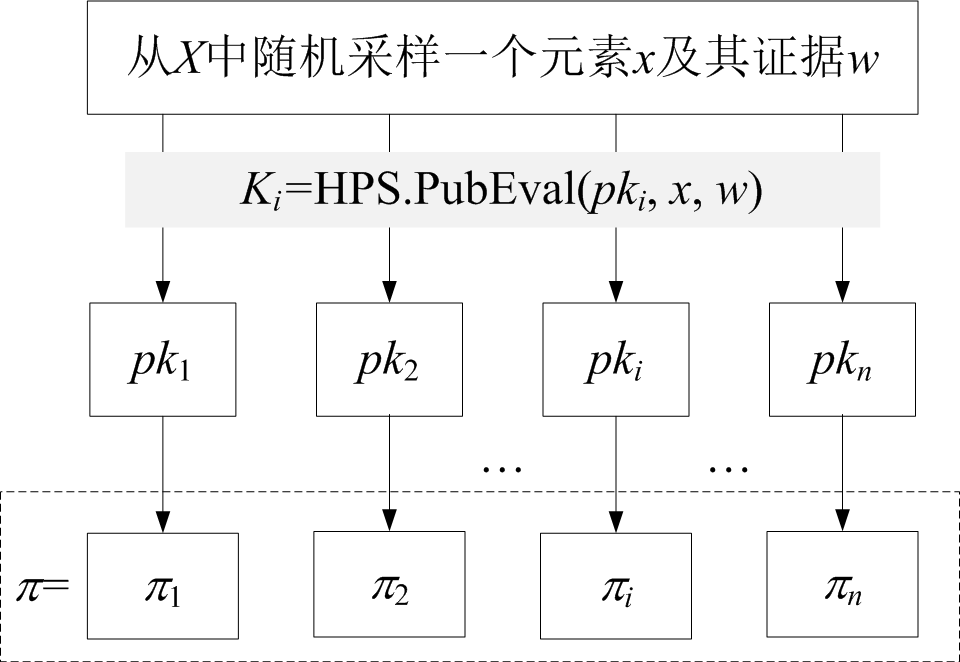
\includegraphics[width=0.5\textwidth]{./figure/ParallelHPS.png}
\end{center}
\caption{并行化哈希证明系统构造示意图}\label{figure:ParallelHPS}
\end{figure}

\medskip\noindent\textbf{基于DDH假设的一次有损过滤器.} 令$(\mathbb{G}, q, g)$是一个有限循环群, $\mathsf{CH}: \{0, 1\}^* \times \mathcal{R}_{\text{CH}} \rightarrow \mathbb{Z}_q$表示一个变色龙哈希函数. 利用同态矩阵加密和变色龙哈希函数的思想, 可以设计一个$(\mathbb{Z}_q^n, \log q)$-一次有损过滤器, 其标签空间与变色龙哈希函数的定义域相同, 即$\mathcal{T} =  \{0, 1\}^* \times \mathcal{R}_{\text{CH}}$.  设计的基本思路是构造一个如图~\ref{figure:DDH-LF}所示的公钥矩阵$E$, 其中$r_i, s_i\sample \mathbb{Z}_q$, $b^*$可以看作是一个嵌入公钥矩阵$E$中的有损标签的变色龙哈希函数值$b^* = \mathsf{CH}(t_a^*, t_c^*)$计算而来. 
\begin{figure}[!hbtp]
\begin{center}
\[
E = \left(
\begin{array}{llll}
g^{r_1s_1}\cdot g^{-b^*} & g^{r_1s_2}               & \cdots & g^{r_1s_n}\\
g^{r_2s_1}               & g^{r_2s_2}\cdot g^{-b^*} & \cdots & g^{r_2s_n}\\
\vdots                   & \vdots                   & \ddots & \vdots    \\
g^{r_ns_1}               & g^{r_ns_2}               & \cdots & g^{r_ns_n}\cdot g^{-b^*}\\
\end{array}
\right)
\]
\end{center}
\caption{一次有损过滤器的公钥矩阵}\label{figure:DDH-LF}
\end{figure}

对于OT-LF定义域上的任意元素$X = (X_1, X_2, \ldots, X_n) \in \mathbb{Z}_q^n$和任意标签$b \in \mathbb{Z}_q$, OT-LF的运算方式为$y = X\cdot (E \otimes g^{bI})$. 其中$I$表示$n \times n$阶单位矩阵, 运算符$\otimes$表示矩阵对应位置元素两两相乘. 对于矩阵$E = (E_{i,j}) \in \mathbb{G}^{n \times n}$, $X\cdot E$的运算方式为
\[
X \cdot E = \left(\Pi_{i=1}^n E_{i, 1}^{X_i}, \Pi_{i=1}^n E_{i, 2}^{X_i},\ldots, \Pi_{i=1}^n E_{i, n}^{X_i}\right).
\]
由此可见, 当$b = b^*$时, OT-LF的值由$g^{\sum_{i=1}^n r_iX_i}$完全确定了, 此时OT-LF工作在有损模式下. 因此, 对于有损标签, OT-LF值泄漏$X$的信息量不超过$\log q$比特. 当$b \neq b^*$时, $X_i$由$g^{\sum_{i=1}^n r_iX_i}\cdot g^{(b - b^*)X_i}$完全确定, 此时OT-LF工作在单射模式下. 此外, 利用变色龙哈希函数的性质, 对于任意$t_a \in \{0, 1\}^*$, 可以利用变色龙哈希函数的陷门及$(t_a^*, t_c^*)$计算出另一个有损标签$(t_a, t_c)$使得$\mathsf{CH}(t_a, t_c) = \mathsf{CH}(t_a^*, t_c^*)$.

\begin{note}
根据上述基于DDH问题构造的1-universal HPS和OT-LF的性质, 我们可以得到一个容忍密钥泄漏量为$L(1/2 - o(1))$的BKL-CCA安全公钥加密方案. 类似地, 基于DCR问题也可构造容忍同等水平密钥泄漏的BKL-CCA安全公钥加密方案. 然而, 要到达最优密钥泄漏量$L(1 - o(1))$, 我们需要基于一些特殊的困难问题, 如加强的子群不可区分问题 (Refined Subgroup Indistinguishability Problem)~\cite{Qin-PKC-2014}, 来设计哈希证明系统及一次有损过滤器.
\end{note}


\subsection{CQX18方案}
2018年, Chen等人~\cite{Chen-TCS-2018,Chen-CTRSA-2018}提出规则有损函数的概念并用于设计抗泄漏密码学原语, 包括抗泄漏单向函数、抗泄漏消息认证码、抗泄漏密钥封装方案等.
\subsubsection{规则有损函数及扩展}
\medskip\noindent\textbf{规则有损函数.} 下面给出规则有损函数(Regular Lossy Functions)的形式化定义.
\begin{definition}[规则有损函数]
假设定义域为$2^{n(\kappa)}$, 其中$n(\kappa) = \mathsf{poly}(\kappa)$. 定义$\nu(\kappa) \leq 2^{n(\kappa)}$表示非单射集合, $2^{\tau(\kappa)} \leq 2^{n(\kappa)}$表示像空间. 一个$(\nu, \tau)$-RLFs由以下四个多项式时间算法组成并满足以下性质:
\begin{itemize} \itemsep 1pt \parskip 0pt \parsep 0pt
\item $\mathsf{Setup}(\kappa)$: 以安全参数$\kappa$为输入, 输出公开参数$pp$, 其中$pp$包含对求值公钥空间$EK$, 定义域$X$和值域$Y$的描述. 

\item $\mathsf{GenNormal}(pp)$: 以公开参数$pp$为输入, 输出求值公钥$ek$. 
	$f_{ek}(\cdot): X \rightarrow Y$是一个$\nu$-规则函数. 

\item $\mathsf{GenLossy}(pp)$: 以公开参数$pp$为输入, 输出求值公钥$ek$.  
	$f_{ek}(\cdot): X \rightarrow Y$是一个有损函数, 像空间最大为$2^\tau$.损耗定义为$n - \tau$. 

\item $\mathsf{Eval}(ek, x)$: 以求值公钥$ek$和原像$x \in X$为输入, 输出$y \leftarrow f_{ek}(x)$. 
\end{itemize}

\begin{trivlist}
\item \textbf{模式不可区分性.} 对于任意公开参数$pp \leftarrow \mathsf{Setup}(\kappa)$, $\mathsf{GenNormal}(pp)$和$\mathsf{GenLossy}(pp)$输出的求值公钥在计算意义下不可区分.
\end{trivlist}
\end{definition}

图~\ref{figure:ch5-RLFs}给出了规则有损函数的示意图. 在$\nu$-标准模式中, 每个像都有$2^{\nu}$相同大小的原像空间. 相应地, 像空间也缩减为$2^{n - \nu}$. 在$\tau$-有损模式中, 像空间大小仅有$2^{\tau}$, 并且$2^n \gg 2^{\tau}$. 

\begin{figure}[!hbtp]
\begin{center}
\begin{tikzpicture}

\node [textnode, name=normal] {标准模式\\$\mathsf{GenNormal}(\kappa) \rightarrow ek$}; 
\node [shapenode, name=domain1, circle, draw=gray!50, fill=gray!50, minimum size=4em, 
	right of = normal, xshift=8em] {$X$}; 
\node [shapenode, name=range1, circle, draw=blue!20, fill=blue!20, minimum size=4em, right of = domain1, xshift=12em] {$Y$};

\node [shapenode, name=x, circle, draw=gray!50, fill=red!50, right of = domain1, inner sep =0, 
	minimum size=1em, xshift=0.8em] {};
\node [shapenode, name=y, circle, draw=black, fill=black, left of = range1, inner sep = 0, minimum size=0.1em, xshift=-1em] {}; 
\draw ($(x.east)+(-0.5em, 0em)$) edge[-] (y);
\draw ($(x.east)+(-0.5em, 0.3em)$) edge[-] (y); 
\draw ($(x.east)+(-0.5em, -0.3em)$) edge[-] (y); 

\node [shapenode, name=x5, circle, draw=gray!50, fill=red!50, right of = domain1, inner sep =0, 
minimum size=1em, xshift=1em, yshift=1.1em] {};
\node [shapenode, name=y5, circle, draw=black, fill=black, left of = range1, inner sep = 0, 
minimum size=0.1em, xshift=-1.2em, yshift=0.6em] {}; 
\draw ($(x5.east)+(-0.5em, 0em)$) edge[-] (y5);
\draw ($(x5.east)+(-0.5em, 0.3em)$) edge[-] (y5); 
\draw ($(x5.east)+(-0.5em, -0.3em)$) edge[-] (y5); 

\node [shapenode, name=x6, circle, draw=gray!50, fill=red!50, right of = domain1, inner sep =0, 
minimum size=1em, xshift=1em, yshift=-1.1em] {};
\node [shapenode, name=y6, circle, draw=black, fill=black, left of = range1, inner sep = 0, 
minimum size=0.1em, xshift=-1.2em, yshift=-0.6em] {}; 
\draw ($(x6.east)+(-0.5em, 0em)$) edge[-] (y6);
\draw ($(x6.east)+(-0.5em, 0.3em)$) edge[-] (y6); 
\draw ($(x6.east)+(-0.5em, -0.3em)$) edge[-] (y6); 

\node [textnode, name = v, right of = x, xshift = 5em, yshift=3.5em] {$\red{v}$-regular}; 

\node [name=indistinguishable, below of=normal, yshift=-1em] {$\approx_c$};

\draw ($(indistinguishable.east)+(4em, 0em)$) edge[dashed] ($(indistinguishable.east)+(22em, 0em)$);

\node [textnode, name = lossy, below of=indistinguishable, yshift=-4em] 
	{$\mathsf{GenLossy}(\kappa) \rightarrow ek$\\有损模式};  
\node [shapenode, name=domain2, circle, draw=gray!50, fill=gray!50, minimum size=4em, 
	right of = lossy, xshift=8em] {$X$}; 
\node [shapenode, name=range2, circle, draw=blue!20, fill=blue!20, minimum size=4em, 
	right of = domain2, xshift=12em] {\quad$Y$}; 
\node [shapenode, name=image, circle, draw=blue!60, fill=blue!60, minimum size=1em, left of = range2, xshift=-1em] {}; 

\node [shapenode, draw=black, circle, fill=black, name=xlossy, right of = domain2, 
	inner sep=0, minimum size=0.1em, xshift=1em] {};
\node [shapenode, draw=black, circle, fill=black, name=ylossy, left of = range2, 
	inner sep=0, minimum size=0.1em, xshift=-1em] {}; 
\draw (xlossy) edge[connect] node[auto] {$f_{ek}$} (ylossy);

\node [shapenode, draw=black, circle, fill=black, name=x1, right of = domain2, inner sep = 0, 
	minimum size=0.1em, xshift=0.4em, yshift=1.5em] {};
\node [shapenode, draw=black, circle, fill=black, name=x2, right of = domain2, inner sep = 0, 
	minimum size=0.1em, xshift=0.8em, yshift=0.75em] {};

\node [shapenode, draw=black, circle, fill=black, name=x3, right of = domain2, inner sep = 0, 
	minimum size=0.1em, xshift=0.8em, yshift=-0.75em] {};
\node [shapenode, draw=black, circle, fill=black, name=x4, right of = domain2, inner sep = 0,  
	minimum size=0.1em, xshift=0.4em, yshift=-1.5em] {};

\draw (x1) edge[-, bend left=45] (ylossy);
\draw (x2) edge[-, bend left=30] (ylossy);
\draw (x3) edge[-, bend left=-30] (ylossy);
\draw (x4) edge[-, bend left=-45] (ylossy);

\node [textnode, name=domainsize, below of = domain2, yshift=-4em] {$2^n$}; 
\node [textnode, right of = domainsize, xshift=4em] {$\gg$}; 
\node [textnode, name=imagesize, below of = image, yshift=-4em] {$2^{\red{\tau}} = 2^{n-\ell}$};
\end{tikzpicture}
\end{center}
\caption{规则有损函数(RLFs)示意图}\label{figure:ch5-RLFs}
\end{figure}

\begin{note}
规则有损函数可以看作是有损函数的一般化形式. 当$\nu = 1$时, 规则有损函数即是有损函数. ``规则有损(regular lossy)''这一概念在~\cite{KPS-CRYPTO-2013,Seurin-PKC-2014}等文献中也有介绍. 但是与本文中的概念区别较大. 前者要求有损模式是规则有损的, 而本文要求的是在标准模式中是(近似)规则有损的. 对于一个近似规则有损函数, 在标准模式下, 函数值的熵几乎保存了原像的熵, 可以很容易得到如下的引理:
\begin{lemma}\label{lemma:preserve}
假设$f: D \rightarrow R$是一个$\nu$-到-1规则函数, $X$是定义域$D$熵的一个随机变量, 则有: 
\begin{equation*}
	\minentropy(f(X)) \geq \minentropy(X) - \log \nu
\end{equation*} 
\end{lemma}
\end{note}

\medskip\noindent\textbf{全除一规则有损函数.} 类似于全除一有损函数(ABO-LFs), 规则有损函数也可以推广为全除一规则有损函数(ABO-RLFs), 其形式化定义见定义~\ref{definition:ch5-ABO-RLFs}.
\begin{definition}[全除一有损函数]\label{definition:ch5-ABO-RLFs}
在定义中, 参数$n$, $\nu$, $\tau$的含义同规则有损函数, $B$表示分支空间. 一个$(\nu, \tau)$-ABO-RLFs包含以下三个多项式时间算法并满足以下性质:
\begin{itemize} \itemsep 1pt \parskip 0pt \parsep 0pt
\item $\mathsf{Setup}(\kappa)$: 以安全参数$\kappa$为输入, 输出公共参数$pp$, 其中$pp$包含对求值密钥空间$EK$, 分支空间$B$, 定义域$X$和值域$Y$的描述. 

\item $\mathsf{Gen}(pp, b^*)$: 以公开参数$pp$和分支$b^* \in B$为输入, 输出一个求值密钥$ek$. 
对于任意$b \neq b^*$, $f_{ek,b}(\cdot)$是一个从$X$到$Y$的$\nu$-规则函数, 
	而$f_{ek,b^*}(\cdot)$是一个从$X$到$Y$的有损函数, 其像空间大小最多为$2^{\tau}$.

\item $\mathsf{Eval}(ek, b, x)$: 以求值密钥$ek$, 分支$b \in B$和$x \in X$为输入, 输出$y \leftarrow f_{ek, b}(x)$. 
\end{itemize}

\begin{trivlist}
\item \textbf{隐藏有损分支性质.} 对于任意$b_0^*, b_1^* \in B \times B$, $\mathsf{Gen}(pp, b_0^*)$输出的求值密钥$ek_0$和$\mathsf{Gen}(pp, b_1^*)$输出的求值密钥$ek_1$在计算上是不可区分的. 
	are computationally indistinguishable.
\end{trivlist}
\end{definition}

图~\ref{figure:ch5-ABO-RLFs}给出了全除一有损函数的示意图. 由图示可知, 每个求值函数都会额外输入一个分支$b$,并且有损分支$b^*$隐藏于求值密钥$ek$中. 当$b = b^*$时, 函数才处于有损模式, 其他情况都是规则模式. 
\begin{figure}[!hbtp]
\begin{center}
\begin{tikzpicture}
\node [textnode, name=Gen] {$\mathsf{Gen}(\lambda, b^*) \rightarrow ek$};

\node [textnode, name=dummy, below of=Gen, yshift=-3cm] {$\dots$}; 
\node [textnode, name=F1, left of=dummy, xshift=-5em, yshift=4em] {$f_{ek, b_1}(\cdot)$}; 
\node [textnode, name=F2, left of=dummy, xshift=-3em, yshift=2.5em] {$f_{ek, b_2}(\cdot)$}; 
\node [textnode, name=F3, right of=dummy, xshift=3em, yshift=2.5em] {$f_{ek, \red{b^*}}(\cdot)$}; 
\node [textnode, name=F4, right of=dummy, xshift=5em, yshift=4em] {$f_{ek, b_i}(\cdot)$};  

\draw (Gen) edge[connect] (F1);
\draw (Gen) edge[connect] (F2);
\draw (Gen) edge[connect, dashed, color=red] (F3);
\draw (Gen) edge[connect] (F4);
\draw (Gen) edge[connect] (dummy);

\node [textnode, name=hidden, right of = Gen, xshift=15em, yshift=-4em] {$b^*$隐藏于求值公钥$ek$}; 
\end{tikzpicture}
\begin{displaymath}
f_{ek,b}(\cdot) = \left\{ \begin{array}{ll}
	\text{lossy} & b = b^*\\
 	\text{regular} & b \neq b^*\\
\end{array} \right.
\end{displaymath}
\end{center}
\caption{全除一规则有损函数(ABO-RLFs)示意图}\label{figure:ch5-ABO-RLFs}
\end{figure}

\medskip\noindent\textbf{一次规则有损过滤器.} 在ABO-RLFs中, 求值公钥$ek$完全确定了有损分支$b^*$的值. 因此, 在归约证明中, 有损分支需要提前选取, 并不适应于自适应攻击的敌手环境. 类似前面的OT-LFs, 我们可以将RLFs推广到一次规则有损过滤器(One-Time Regular Lossy Filters, 简称OT-RLFs). OT-RLFs的形式化定义见定义~{definition:ch5-OT-RLFs}.
\begin{definition}[一次规则有损过滤器]\label{definition:ch5-OT-RLFs} 
一个$(\nu, \tau)$-OT-RLFs包含以下四个多项式时间算法并满足以下性质:
\begin{itemize}\itemsep 1pt \parskip 0pt \parsep 0pt
\item $\mathsf{Setup}(\kappa)$: 以安全参数$\kappa$为输入, 
输出公开参数$pp$, 其中$pp$包含对求值密钥空间$EK$, 
分支集合$B = B_c \times B_a$ (其中, $B_c$是核心分支集合, $B_a$是辅助输入分支集合), 定义域$X$和值域$Y$的描述. 

\item $\mathsf{Gen}(pp)$: 以公开参数$pp$为输入, 输出一个求值密钥$ek$和一个陷门$td$. 分支集合$B$包含两个不相交的子集: 规则分支集合$B_\text{normal}$和有损分支集合$B_\text{lossy}$. 
	对于规则分支集合中的任意分支$b \in B_\text{normal}$, $f_{ek, b}(\cdot)$确定了一个从$X$到$Y$的$\nu$-规则函数. 对于有损分支集合中的任意分支$b \in B_\text{lossy}$, $f_{ek, b}(\cdot)$确定了一个从$X$到$Y$且像空间最大为$2^{\tau}$的有损函数.

\item $\mathsf{SampLossy}(td, b_a)$: 以陷门$td$和一个辅助分支$b_a$为输入, 输出一个核心分支$b_c$, 使得$b = (b_c, b_a)$是集合$B_\text{lossy}$中的一个有损分支.

\item $\mathsf{Eval}(ek, b, x)$: 以求值密钥$ek$, 分支$b \in B$和元素$x \in X$为输入, 输出$y \leftarrow f_{ek, b}(x)$.
\end{itemize}

\begin{trivlist}
\item \textbf{Indistinguishability.} 对于任意辅助分支$b_a \in B_a$, 
	由算法生成的核心分支$b_c \leftarrow \mathsf{SampLossy}(td, b_a)$与随机选取的核心分支$b_c \sample B_c$在计算意义下是不可区分的.

\item \textbf{Evasiveness.} 对于任意PPT敌手, 在给定一个有损分支的条件下, 再生成一个新的有损分支是困难的.
\end{trivlist} 
\end{definition}

\begin{remark}
规则有损函数的几个相关概念之间存在一定的联系. 我们知道, ABO-RLFs是RLFs的推广. 实际上, 若存在一个$(\nu, \tau)$-ABO-RLFs函数族, 我们只需要把ABO-RLFs的分支标签作为RLFs的求值密钥参数, 即可以得到一个$(\nu, \tau)$-RLFs函数族. 相反, 类似LTFs与ABO-LTFs的转化关系~\cite{PW-STOC-2008}, 若存在一个$(\nu, \tau)$-RLFs函数族, 则必然存在一个分支集合为$B = \{0, 1\}$的$(\nu, \tau)$-ABO-RLFs函数族. 进一步, 可以推广到分支集合为$B = \{0, 1\}^\ell$的$(\nu, \ell\tau)$-ABO-RLFs函数族. 此外, 根据文献~\cite{Qin-PKC-2014}, 一个$(\nu, \tau)$-ABO-RLFs函数族结合一个变色龙哈希函数, 可以构造一个$(\nu, \tau)$-OT-RLFs函数族. 
\end{remark}

\subsubsection{全除一规则有损函数的具体构造}
本节分别基于DDH问题和DCR问题, 介绍ABO-RLFs函数族的两种具体构造. 

\medskip\noindent\textbf{基于DDH的ABO-RLFs.} 首先回顾群上的伪随机矩阵生成算法$\mathsf{GenConceal}$. 该算法的输入是两个正整数$n$和$m$ (其中$n \geq m$), 输出是一个群元素构成的秩为1的$n \times m$矩阵$\mathbb{G}^{n \times m}$且与随机选取的$n \times m$矩阵不可区分. 该算法的具体执行过程如下: 
\begin{itemize} \itemsep 1pt \parskip 0pt \parsep 0pt
	\item 随机选择两个向量$\mathbf{r} = (r_1, \dots, r_n) \leftarrow \mathbb{Z}_p^n$和$\mathbf{s} = (s_1, \dots, s_m) \leftarrow \mathbb{Z}_p^{m}$. 

	\item 令$\mathbf{V} = \mathbf{r} \otimes \mathbf{s} = \mathbf{r}^t\mathbf{s} \in \mathbb{Z}_p^{n \times m}$表示$\mathbf{r}$与$\mathbf{s}$的外积. 

	\item 输出$\mathbf{C} = g^\mathbf{V} \in \mathbb{G}^{n \times m}$作为concealer matrix.   
\end{itemize} 

\begin{lemma}[\cite{PW2008}]
令$n, m = \mathsf{poly}(\lambda)$.在DDH假设下, 矩阵$\mathbf{C} = g^\mathbf{V} \leftarrow \mathsf{GenConceal}(n, m)$ 在空间$\mathbb{G}^{n \times m}$上是伪随机的.   
\end{lemma}

基于DDH假设的ABO-RLFs构造如下:
\begin{construction}[基于DDH的ABO-RLFs]\label{construction:DDH-ABO-RLFs}  
\begin{itemize} \itemsep 1pt \parskip 0pt \parsep 0pt
\item $\mathsf{Setup}(\kappa)$: 以安全参数$\kappa$为输入, 运行$(\mathbb{G}, g, p) \leftarrow \mathsf{GroupGen}(\lambda)$, 
	输出公开参数$pp = (\mathbb{G}, g, p)$和分支空间$B = \mathbb{Z}_p$.  

\item $\mathsf{Gen}(pp, b^*)$: 以公开参数$pp$和分支$b^* \in \mathbb{Z}_p$为输入, 
调用算法$\mathsf{GenConceal}(n, m)$生成矩阵$\mathbf{C} = g^\mathbf{V} \in \mathbb{G}^{n \times m}$, 
	输出求值密钥$ek = g^\mathbf{Y} = g^{\mathbf{V} - b^* \mathbf{I}'}$, 
	其中$\mathbf{I}' \in \mathbb{Z}_p^{n \times m}$, 即, 第$i$列向量是标准的单位向量$\mathbf{e}_i \in \mathbb{Z}_p^n$, 其中$i \leq n$, 而余下的列向量为零向量. 

\item $\mathsf{Eval}(ek, b, \mathbf{x})$: 以求值密钥$ek = g^\mathbf{Y}$, 
分支$b \in \mathbb{Z}_p$和元素$\mathbf{x} \in \mathbb{Z}_p^n$为输入, 
	输出$\mathbf{y} = g^{\mathbf{x}(\mathbf{Y}+b\mathbf{I}')} = g^{\mathbf{x}(\mathbf{V}+(b-b^*)\mathbf{I}')} 
	\in \mathbb{G}^{m}$.    
\end{itemize}
\end{construction}

\begin{lemma}
	在DDH假设下, 构造~\ref{construction:DDH-ABO-RLFs}是一个$(p^{n-m}, \log p)$-ABO-RLFs, 其中$n > 1$.
\end{lemma}
\begin{proof}
对于任意$b \neq b^*$, $(\mathbf{V}, b)$确定了一个$p^{n-m}$-到-1函数, 这是因为矩阵$(\mathbf{Y}+b\mathbf{I}')$的秩是$m$, 对于每个$y \in \mathbb{G}^m$, 其解空间大小为$p^{n-m}$. 
当$b = b^*$时, 每个输出结果$\mathbf{y}$的形式是$g^{r'\mathbf{s}}$, 其中$r' = \mathbf{x} \mathbf{r}^t \in \mathbb{Z}_p$. 因为$\mathbf{s}$由函数索引$\mathbf{V}$确定, 所以由$(\mathbf{V}, b^*)$确定的每个函数最多有$p$个不同的输出结果. 故, 损耗为$(n-1) \log p$.  
	
在DDH假设下, 通过归约可以证明隐藏有损分支性质: 对于任意分支$b^* \in \mathbb{Z}_p$, $\mathsf{Gen}(\lambda, b^*)$输出的求值密钥矩阵与$\mathbb{G}^{n \times m}$上的随机矩阵在计算意义下是不可区分的. 
\end{proof}

\begin{remark}
在构造中, 参数$n$用于控制定义域的大小, 而参数$m$用于调节ABO分支的规则性. 
当$m = n$时, ABO分支是单射的, 故上述构造方案变成了标准的ABO-LFs. 

在基于DDH的ABO-LTF构造方案中~\cite{PW-STOC-2008}, 定义域限制在$\{0,1\}^n$且$m$必须大于$n$才能保证函数可求逆. 在上述构造中, 由于ABO-RLF不需要可求逆的性质, 在不改变求值密钥矩阵大小的情况下, 定义域可以由$\{0,1\}^n$扩展到$\mathbb{Z}_p^n$. 特别地, ABO-RLF不需要单射性质, 所以矩阵参数$m$可以小于$n$. 在基于矩阵的构造中, 求值密钥大小和计算开销的复杂性取决于参数$n$和$m$. 因此, 与基于DDH的ABO-LTFs相比, ABO-RLFs允许的输入空间更大, 计算效率更高.
\end{remark}   

类似地, 利用Hemenway和Ostrovsky的方法~\cite{HO-PKC-2012b}, 可以将上述基于DDH的构造方案扩展到基于eDDH的构造, 而eDDH问题包含了DDH、QR和DCR等问题. 所以, 上述构造也蕴含了基于DCR的ABO-RLFs. 尽管如此, 直接基于DCR假设, 可以构造出更高效的ABO-RLFs.

\medskip\noindent\textbf{基于DCR的ABO-RLFs.} 基于DCR假设的ABO-RLFs构造如下:
\begin{construction}[基于DCR的ABO-RLFs]\label{construction:ch5-DCR-ABO-RLFs}  
\begin{itemize} \itemsep 1pt \parskip 0pt \parsep 0pt
	\item $\mathsf{Setup}(\kappa)$: 运行$N \leftarrow \mathsf{GenModulus}(\lambda)$生成RSA模$N$, 
随机选择$z \in \mathbb{Z}_N$并计算$g =z^{2N} \mod N^2$, 输出公开参数$pp = (N, y)$, 并令分支空间为$B = \mathbb{Z}_N$.  
	
	\item $\mathsf{Gen}(pp, b^*)$: 以公开参数$pp$和有损分支$b^* \in \mathbb{Z}_N$为输入, 随机选择$r$ in $\mathbb{Z}_N$, 计算并输出求值密钥$ek=g^r(1+N)^{-b^*}$. 
	
	\item $\mathsf{Eval}(ek, b, x)$: 以求值密钥$ek$, 分支$b \in \mathbb{Z}_N$和元素$x \in \{0, \cdots,\lfloor N^2/4\rfloor\}$为输入, 输出$y = [ek/(1+N)^{b}]^x = g^{rx}(1+N)^{(b-b^*)x} \in \mathbb{Z}_{N^2}$.    
\end{itemize}
\end{construction}

\begin{lemma}
	基于DCR假设, 构造方案~\ref{construction:ch5-DCR-ABO-RLFs}是一个$(1, \phi(N)/4)$-ABO-RLFs函数族.
\end{lemma}
\begin{proof}
	对于任意$b \neq b^*$, $f_{ek, b}$是一个单射函数, 这是因为$g$以压倒性的概率是$2N$次剩余群的一个生成元. 
令$\phi$表示欧拉函数. 则$g$的阶至少为$\phi(N)/4$, $g^r(1+N)^{b-b^*}$的阶至少为$N\phi(N)/4$. 
当$b = b^*$时, 每个输出结果$g^{rx}$是一个$2N$次剩余元素. 因此, 所有像元素至多为$\phi(N)/4$个, 损耗至少为$\log N$.  
	
	隐藏有损分支性质源于Paillier加密方案基于DCR假设的安全性~\cite{Paillier-EUROCRYPT-1999}: 算法$\mathsf{Gen}(pp, b^*)$的输出结果实际上是Paillier方案选择随机数$r$加密消息$b^*$的一密文. 因此, 对于任意$b_0^*, b_1^* \in \mathbb{Z}_N$, $\mathsf{Gen}(pp, b_0^*)$的输出结果和$\mathsf{Gen}(pp, b_1^*)$的输出结果在计算意义下是不可区分的.
由于规则损耗参数为$\nu = 1$, 所以方案~\ref{construction:ch5-DCR-ABO-RLFs}实际上是一个ABO-LFs函数族. 
\end{proof}

\subsubsection{全除一规则有损函数的通用构造}
由于全除一规则有损函数可以由规则有损函数构造. 为此, 本节重点介绍如何基于哈希证明系统构造规则有损函数.

\medskip\noindent\textbf{基于哈希证明系统的一般构造.}
2012年, Wee提出利用对偶哈希证明系统构造有损陷门函数. 对偶哈希证明系统的概念可以参考文献~\cite{Wee-EUROCRYPT-2012}或第6章定义~\ref{definition:DualHPS}. 假设$(\mathsf{H}, SK, PK, X, L, W, \Pi, \alpha)$是对偶哈希证明系统的公开参数, 其中$\mathsf{H}: X \times SK \rightarrow \Pi$.
Wee基于对偶哈希证明系统的有损陷门函数$f$构造方式如公示~\eqref{eqn:twist-HPS}所示. 
\begin{equation}\label{eqn:twist-HPS}
	f_x(sk) = \alpha(sk) || \mathsf{H}_{x}(sk)
\end{equation}
在上述构造中, 哈希证明系统的密钥$sk \in SK$充当了有损陷门函数的定义域, 而子集成员$x \in X$充当了函数的求值密钥. 当$x \in X \setminus L$时, 根据对偶哈希证明系统的可逆性质, $f_x$是单射函数且可逆; 根据对偶哈希证明系统的仿射性质, 当$x \in L$时, 函数$f_x$是有损函数. 基于子集合成员判定困难问题, 这两种模式在计算意义下是不可区分的. 

有趣的是, 利用上述构造方式, 可以基于任意的哈希证明系统构造规则有损函数. 由于规则有损函数比有损陷门函数的性质要弱, 仅需要哈希证明系统的仿射性质即可, 并不需要哈希证明其他额外的性质, 比如平滑性、一致性、可逆性等. 令$(\mathsf{H}, SK, PK, X, L, W, \Pi, \alpha)$是哈希证明系统的一个公开参数. 对于任意$x \in X \setminus L$, 假设$f_x(sk) = \alpha (sk) || \mathsf{H}_x(sk)$是一个从定义域$SK$到值域$\Pi$的$\nu$-到-1函数. 我们有以下引理 
\begin{lemma}
基于子集成员判定问题假设, 公示~\eqref{eqn:twist-HPS}是一个$(\nu, \log |\textup{Img}(\alpha)|)$-规则有损函数. 
\end{lemma} 

\begin{proof}
标准模式的正确性源于$f_x(\cdot)$是一个$\nu$-到-1函数. 
有损模式的损耗性源于哈希证明系统的仿射性质. 对于任意$x \in L$, $\textup{Img}(f_x) = \textup{Img}(\alpha)$. 两种模式的不可区分性可以归约到子集成员判定问题的困难性. 
\end{proof}

至此, 利用哈希证明系统构造全除一规则有损函数可以通过以下两步实现: (1)利用哈希证明系统构造一个规则有损函数族; (2) 将具有二元分支空间$\{0, 1\}$的规则有损函数放大到分支空间为$\{0,1\}^\ell$的全除一规则有损函数. 然而, 第二步扩大分支空间的效率并不高, 需要进行$\ell$次独立地规则有损函数计算, 且损耗量也会降低.  

\medskip\noindent\textbf{基于哈希证明系统的高效构造.} 在前面的构造方案中, 哈希证明系统所基于的子集成员判定问题没有任何代数结构限制. 如果子集成员判定问题具有一定的代数结构, 则可以构造更加高效的ABO-RLFs函数族. 构造的主要思想是利用. 
 
\begin{trivlist}
\item \textbf{代数子集成员判定问题(ASMPs).} 该问题是一种特殊的子集成员判定问题$(X, L)$, 满足以下几个性质: 
\begin{enumerate}\itemsep 1pt \parskip 0pt \parsep 0pt
	\item $X$是一个有限阿贝尔群, $L$是$X$的一个子群. 
	\item 商群$H = X/L$是一个阶为$p = |X|/|L|$的循环群. 
\end{enumerate}
基于上述性质, 我们可以推出以下两个实用的结论: 
\begin{itemize}\itemsep 1pt \parskip 0pt \parsep 0pt
	\item 令$\overline{a} = aL$, 其中$a \in X \backslash L$是$H$的一个生成元, 
		则陪集$(aL, 2aL, \dots, (p-1)aL, paL = L)$构成了$X$的一个划分. 

	\item 对于任意$x \in L$, $ia + x \in X \backslash L$, 其中$1 \leq i < p$. 
\end{itemize}     

ASMPs问题的困难性同SMPs问题一样, 要求集合$L$和$X \backslash L$上的元素分布在计算意义下是不可区分的. $L$的密度定义为$\rho = |L|/|X|$. 当$\rho$是可忽略时, $U_L \approx_c U_{X \backslash L}$等价于 
$U_L \approx_c U_{X}$. 此时, $U_{X \backslash L}$和$U_X$统计距离接近. 
当$\rho$已知时, $U_L \approx_c U_{X \backslash L}$意味着$U_L \approx_c U_X$, 这是因为$U_X$可由$U_L$, $U_{X \backslash L}$和$\rho$重构出来.
\end{trivlist} 

\begin{remark}
ASMP问题具有一般性, 可由DDH、$d$-linear、QR和DCR等假设构造. 此外, ASMP问题可以看作是满足性质2的加强子群成员判定问题.  在实际应用中, 性质2可以放宽至$H$包含一个循环子群. 
\end{remark}

\begin{trivlist}
\item \textbf{与(加强)子群不可区分问题的比较.} 2010年, Brakerski和Goldwasser~\cite{BG-CRYPTO-2010}提出子群不可区分问题(简称SIPs问题). SIPs问题定义在一个阿贝尔群$X$和子群$L$上. 此外, SIPs要求$X$同构于两个群的直积, 即$X \simeq L \times M$且$\mathsf{gcd}(\text{ord}(L), \text{ord}(M)) = 1$. 2014年, Qin和Liu~\cite{Qin-PKC-2014}提出加强的子群不可区分问题(简称RSIPs), 进一步要求$M$也是一个循环子群. 与RSIPs问题相比, ASMPs问题仅要求商群$X/L$是循环的. 因此, ASMP问题要强于RSIP问题, 按理也比SIP问题强, 因为SIP问题无法由DDH和$d$-linear等问题构造. 由此可见, 代数子集合成员判定假设要弱于RSIP和SIP等假设..    
\end{trivlist}

下面给出基于ASMP-HPS的ABO-RLF的构造. 
\begin{construction}
假设HPS是一个基于ASMP问题的哈希证明系统, 则ABO-RLF的具体构造如下:   
\begin{itemize} \itemsep 1pt \parskip 0pt \parsep 0pt
	\item $\mathsf{Setup}(\kappa)$: 运行$\text{HPS}.\mathsf{Setup}(\kappa)$生成HPS的公开参数$pp = (\mathsf{H}, SK, PK, X, L, W, \Pi, \alpha)$, 选择商群$H$的一个随机生成元$aL$, 输出公开参数$\hat{pp} = (pp, a)$.    

	\item $\mathsf{Gen}(\hat{pp}, b^*)$: 以公开参数$\hat{pp} = (pp, a)$和一个有损分支$b^* \in \mathbb{Z}_p$为输入, 
运行$(x, w) \leftarrow \text{HPS}.\mathsf{SampYes}(pp)$抽取$L$中的一个随机元素, 
计算求值密钥$ek = -b^*a + x \in X$. 

	\item $\mathsf{Eval}(ek, b, sk)$: 以求值密钥$ek = -b^*a + x$, 分支$b$和$sk$为输入, 
计算并输出$\alpha(sk)||\mathsf{H}_{sk}(ek+ba)$. 该算法定义了$f_{ek,b}(sk):= \alpha(sk)||\mathsf{H}_{sk}(ek+ba)$.  
\end{itemize}
\end{construction}
 
\begin{theorem}
假设$X = \{0,1\}^n$. 对于任意$x \notin L$, 函数$f_x(sk) = \alpha(sk)||\mathsf{H}_x(sk)$是一个$\nu$-规则函数. 上述构造是一个基于代数子集成员判定问题的$(\nu, \log |\textup{Img} \alpha|)$-ABO-RLFs函数族. 
\end{theorem}

\begin{proof}
根据ASMP问题的性质, 当$b \neq b^*$时, $ek + ba= x+(b-b^*)a \notin L$. 此时, $f_{ek,b}(\cdot)$是一个$\nu$-规则函数. 当$b = b^*$时, $ek + ba= x+(b-b^*)a = x \in L$. 此时, $f_{ek,b}(\cdot)$是一个有损函数. 
在安全性方面, 隐藏有损分支性质源于代数子集成员判定问题的困难性, 即对于任意$b_0^*, b_1^* \in \mathbb{Z}_p$, $(-b_0^*a + x) \approx_c (-b_0^*a + u) \equiv u 
\equiv (-b_1^*a + u) \approx_c (-b_1^*a + x)$, 当$u \sample X$. 定理得证!\qed 
\end{proof}

\subsubsection{规则有损函数的应用}
有损陷门函数在标准模式下具有求逆陷门和单射性, 因此可以用于构造公钥加密方案、抗碰撞哈希函数等高级密码学原语. 规则有损函数在这些应用方面似乎无用武之地. 然而, 在泄漏密码学领域, 规则有损函数及其重要的应用价值. Chen等人~\cite{Chen-TCS-2018}指出规则有损函数可以用于构造抗泄漏单向函数(Leakage-Resilient OWFs)、抗泄漏消息认证码(Leakage-Resilient MACs)、抗泄漏和选择密文攻击安全的密钥封装方案(Leakage-Resilient CCA-secure KEM)等高级密码学原语. 下面对这些构造分别作一简要介绍.

\medskip\noindent\textbf{抗泄漏单向函数.} 类似有损陷门函数蕴含一个单向陷门函数, 规则有损陷门函数则蕴含一个抗泄漏单向函数, 有以下定理保证.
\begin{theorem}\label{theorem:LF-to-LROWF}
假设$\text{RLF} = (\mathsf{Setup}, \mathsf{GenInj}, \mathsf{GenLossy}, \mathsf{Eval})$是一个定义在$\{0, 1\}^n$上的规则有损函数族, 其有损模式的像空间大小最多为$2^\tau$. 则$(\mathsf{Setup}, \mathsf{GenInj}, \mathsf{Eval})$是一个$\ell$-抗泄漏单向函数, 其中$\ell \leq n - \tau -\omega(\log \kappa)$. 
\end{theorem}
关于抗泄漏单向函数的形式化定义及安全模型可以参考文献~\cite{Chen-TCS-2018}的附录A.1. 下面简要介绍该定理的证明.
\begin{proof}
我们通过游戏序列的方式组织证明. 令$S_i$表示事件``$\mathcal{A}$在游戏$i$中成功''. 
\begin{trivlist}
\item \textbf{Game 0.} 该游戏是标准的抗泄漏单向函数游戏, 其中挑战者$\mathcal{CH}$与敌手$\mathcal{A}$按以下方式交互: 
    \begin{enumerate} \itemsep 1pt \parskip 0pt \parsep 0pt
        \item 初始化: $\mathcal{CH}$生成(标准模式)求值密钥$ek \leftarrow \mathsf{GenInj}(\kappa)$, 
            随机选择$x^* \sample \{0,1\}^n$并计算$y^* \leftarrow f_{ek}(x^*)$, 然后将$(ek, y^*)$发送给敌手$\mathcal{A}$作为挑战信息. 

        \item 泄漏询问: $\mathcal{A}$可以自适应地进行泄漏询问. 对于任意泄漏询问$\langle g \rangle$, $\mathcal{CH}$返回$g(x^*)$. 

        \item 求逆: $\mathcal{A}$输出$x$, 如果$x = x^*$则$\mathcal{A}$成功.
    \end{enumerate}
    根据定义, 则有: 
    \begin{equation*}
        \mathsf{Adv}_\mathcal{A}(\kappa) = \Pr[S_0]
    \end{equation*}

\item \textbf{Game 1.} 该游戏与Game~0唯一不同之处在于第1步:
    \begin{enumerate} \itemsep 1pt \parskip 0pt \parsep 0pt
        \item 初始化: $\mathcal{CH}$生成(有损模式)求值密钥$ek \leftarrow \mathsf{GenLossy}(\kappa)$. 
    \end{enumerate}  

\item 根据两种模式的不可区分性, 则有: 
\begin{equation*}
    |\Pr[S_1] - \Pr[S_0]| \leq \mathsf{negl}(\kappa)
\end{equation*} 
\end{trivlist}
下面重点分析游戏~1中的概率$\Pr[S_1]$. 假设$ek$是任意一个由$\mathsf{GenLossy}(\kappa)$生成的求值密钥. 对于任意敌手, 成功猜测$x^*$的概率完全由$x^*$的平均极小熵. 特别地, 在已知$y^* \leftarrow f_{ek}(x^*)$和$x^*$的部分泄漏信息条件下, $x^*$的平均极小熵为$2^{-\avminentropy(x^*|(y^*, leak))}$. 由于$f_{ek}(\cdot)$的输出结果最多有$2^\tau$种可能值, 泄漏量最多为$2^\ell$, 则有
    \begin{equation*}
        \avminentropy(x^*|(f_{ek}(x^*), leak)) \geq \minentropy(x) - \tau - \ell = n - \tau - \ell
    \end{equation*} 
由于$n - \tau - \ell \geq \omega(\log \lambda)$, 则$\mathcal{A}(ek, y^*, leak)$输出$x^*$的概率是可忽略的$\mathsf{negl}(\lambda)$. 该结论对于由$\mathsf{GenLossy}$随机生成的求值密钥$ek$也成立. 这就证明了$\Pr[S_1] = \mathsf{negl}(\kappa)$, 从而$\Pr[S_0]$也是可忽略的. 定理得证!\qed 
\end{proof}


\medskip\noindent\textbf{抗泄漏消息认证码.} 消息认证码是一种重要的密码学原语, 在认证协议、公钥加密方案设计等方面具有重要的应用. 关于抗泄漏消息认证码的形式化定义及其安全模型可以参考文献~\cite{Chen-TCS-2018}的附录A.2. 下面介绍如何利用ABO-RLF或者OT-RLF可以构造抗泄漏消息认证码. 利用ABO-RLF构造MAC的主要思路将ABO-RLF的定义域输入看作MAC的密钥, 而将输入的分支看作消息, 其输出作为MAC的标签, 如图~\ref{figure:ch5-LRMAC}所示. 
\begin{figure}
\begin{center}
\begin{tikzpicture}
	\node [name=ingredient, textnode] {Ingredient\\$(v, \tau)$-ABORLF}; 

    \node [name=keygen, right of = ingredient, xshift=10em, shapenode, rounded corners=0.5em, minimum width=5em, minimum height=2em] {$\mathsf{KeyGen}$};
    \node [name=action1, textnode, below of =keygen, yshift=-4em] 
    	{$ek \leftarrow \text{ABORLF}.\mathsf{Gen}(\lambda, 0^d)$\\$k \sample \{0,1\}^n$}; 
    \draw (keygen) edge[->] (action1); 

	\node [name=tag, shapenode, below of = keygen, xshift=-8em, yshift=-10em, 
		rounded corners=0.5em, minimum width=5em, minimum height=2em] {$\mathsf{Tag}$};
	\node [name=m1, textnode, left of=tag, xshift=-5em] {$m$}; 
	\node [name=action2, textnode, below of =tag, yshift=-4em] {$t \leftarrow f_{ek,m}(k)$}; 
	\draw (m1) edge[->] (tag); 	
	\draw (tag) edge[->] (action2); 
	\draw (action1) edge[-] ($(action1.south)+(0em, -2em)$); 
	\draw ($(action1.south)+(0em, -2em)$) edge[-] ($(action1.south)+(-8em, -2em)$); 
	\draw ($(action1.south)+(-8em, -2em)$) edge[->] (tag); 

    \node [name=trick, textnode, below of = keygen, yshift=-11em, color=blue] {$k$ - input\\$m$ - branch\\$t$ - output}; 

	\node [name=vefy, shapenode, right of = keygen, xshift=8em, yshift=-10em, 
		rounded corners=0.5em, minimum width=5em, minimum height=2em] {$\mathsf{Vefy}$};
	\node [name=m2, textnode, right of=vefy, xshift=5em, yshift=0.5em] {$m$};
	\node [name=t, textnode, right of=vefy, xshift=5em, yshift=-0.5em] {$t$};  
	\node [name=action3, textnode, below of =vefy, yshift=-4em] {$t =? f_{ek,m}(k)$}; 
	\draw (m2) edge[->] ($(vefy.east)+(0em,0.5em)$); 	
	\draw (t) edge[->] ($(vefy.east)+(0em,-0.5em)$); 
	\draw (vefy) edge[->] (action3); 
	\draw ($(action1.south)+(0em, -2em)$) edge[-] ($(action1.south)+(8em, -2em)$); 
	\draw ($(action1.south)+(8em, -2em)$) edge[->] (vefy); 
\end{tikzpicture}
\caption{抗泄漏消息认证码构造示意图}\label{figure:ch5-LRMAC}
\end{center}
\end{figure}

\begin{construction}[基于ABO-RLF的抗泄漏消息认证码]\label{construction:ch5-ABORLF-to-MAC}
\begin{itemize} \itemsep 1pt \parskip 0pt \parsep 0pt
\item $\mathsf{Setup}(\kappa)$: 运行$\text{ABORLF}.\mathsf{Setup}(\kappa)$生成RLF的公开参数$pp = (EK, B, X, Y)$, 其中$|X| = 2^n$和$B = \{0,1\}^b$, 运行$\text{ABORLF}.\mathsf{Gen}(pp, 0^b)$生成RLF的求值密钥$ek$, 输出MAC的公开参数$\hat{pp} = (pp, ek)$. 密钥空间、消息空间和认证码空间分别定义为$K = X$、$M = B$和$T = Y$. 

\item $\mathsf{Gen}(\hat{pp})$: 随机选择$k \sample X$作为MAC的密钥. 

\item $\mathsf{Tag}(k, m)$: 以密钥$k$和消息$m$为输入, 计算$t \leftarrow f_{ek, m}(k)$, output $(m, t)$作为消息$m$的认证码. 

\item $\mathsf{Vefy}(k, m, t)$: 如果$t = f_{ek,m}(k)$则输出$1$, 否则输出$0$. 
\end{itemize}
\end{construction}

\begin{theorem}\label{theorem:ch5-ABORLF-to-MAC}
如果ABORLF是一个$(\nu, \tau)$-ABO-RLFs函数族, 则构造方案~\ref{construction:ch5-ABORLF-to-MAC}是一个$\ell$-抗泄漏消息认证码, 其中$\ell \leq \leq n - \tau - \log \nu - \omega(\log \lambda)$. 
\end{theorem}

\begin{proof}
下面通过游戏的方式组织证明. 令$S_i$表示事件``$\mathcal{A}$在游戏$i$中攻击成功''. 
\begin{trivlist}
\item \textbf{Game 0.} 该游戏是消息认证码的抗泄漏一次强伪造安全性游戏. 
    挑战者$\mathcal{CH}$通过以下方式与敌手$\mathcal{A}$交互完成游戏. 
\begin{enumerate} \itemsep 1pt \parskip 0pt \parsep 0pt
\item 承诺和初始化: 敌手$\mathcal{A}$在看到公开参数前, 声明一个目标消息$\langle m^* \rangle$. 
    $\mathcal{CH}$运行$pp \leftarrow \text{ABORLF}.\mathsf{Setup}(\kappa)$和$ek \leftarrow \text{ABORLF}.\mathsf{Gen}(pp, 0^b)$. $\mathcal{CH}$选择$k \sample X$, 计算$t^* \leftarrow f_{ek,m^*}(k)$, 再将$\hat{pp} = (pp, ek)$和$t^*$发送给$\mathcal{A}$. 

\item 学习阶段: $\mathcal{A}$可以自适应地进行泄漏询问. 对于任意泄漏查询$\langle g \rangle$, 只要泄漏量不超过$\ell$, $\mathcal{CH}$返回$g(k)$给$\mathcal{A}$.   

\item 伪造: $\mathcal{A}$输出$(m, t)$. 如果$m \neq m^*$且$t = f_{ek,m}(k)$, 则$\mathcal{A}$成功. 
\end{enumerate}
根据定义, 则有: 
\begin{equation*}
    \mathsf{Adv}_\mathcal{A}(\kappa) = \Pr[S_0]
\end{equation*}

\item \textbf{Game 1.} 该游戏与Game 0的唯一区别是第1步中, $\mathcal{CH}$通过运行$\text{ABORLF}.\mathsf{Gen}(pp, m^*)$替代$\text{ABORLF}.\mathsf{Gen}(pp, b^*)$生成$ek$.  
    根据ABO-RLF隐藏有损分支的性质, Game 0与Game 1在计算上不可区分. 因此有: 
\begin{equation*}
    |\Pr[S_1] - \Pr[S_0]| \leq \mathsf{negl}(\kappa)
\end{equation*}
下面分析事件$S_1$的概率$\Pr[S_1]$. 由于构造的消息认证码唯一, 事件$S_1$实际上等价于$\mathcal{A}$输出$(m, t)$, 其中$m \neq m^*$且$f_{ek, m}(k) = t$.  则消息认证码$t$的条件熵由$\mathcal{A}$的视图$(pp, ek, m, leak, m^*, t^*)$决定. 具体为 
\begin{eqnarray}
\avminentropy(t|view) & = & \avminentropy(t|ek, m, leak, t^*) \label{eqn:MAC-1}\\ 
                    & \geq & \avminentropy(t|ek, m) -\ell - \tau \label{eqn:MAC-2} \\  
                    & \geq & n - \log \nu - \ell - \tau \label{eqn:MAC-3} 
\end{eqnarray}

在上面的推导过程中, 公示~\eqref{eqn:MAC-1}依据事实$t = f_{ek,m}(k)$由$ek$、$m$和$k$决定, 且$k$与$m^*$和$pp$独立. 公式~\eqref{eqn:MAC-2}依据引理~\ref{lemma:chainning-lemma}和泄漏量的上界$\ell$比特, 以及认证码$t^*$最多有$2^{\tau}$个可能的值. 对于任意$m \neq m^*$, $f_{ek,m}(\cdot)$是一个$\nu$-到-1函数. 所以$\mathsf{H}_{\infty}(f_{ek, m}(k)) \geq \mathsf{H}_{\infty}(k) - \log \nu$, 从而公式~\eqref{eqn:MAC-3}成立. 

根据参数选择方式, 则有$n - \log \nu - \ell - \tau \geq \omega(\log \kappa)$. 因此, $\Pr[S_1] \leq \mathsf{negl}(\kappa)$成立.     
\end{trivlist}
综上, 定理得证! \qed. 
\end{proof}

\medskip\noindent\textbf{抗泄漏密钥封装方案.} 类似Qin和Liu在2013年亚密会上提出的抗泄漏公钥加密方案的设计模式, 利用ABO-RLF设计CCA安全的抗泄漏密钥封装方案也额外需要一个哈希证明系统作为封装密钥的工具. 设计思路如图~\ref{figure:ch5-LRKEM}所示. 简单地说, 先利用一个哈希证明系统封装一个(随机)哈希值$\pi$, 再利用ABO-RLF计算$\pi$的知识证明$t$, 类似于Cramer-Shoup方案的指定验证者零知识证明. 这里的$t$也可以看作是密文参数的一个消息认证码. 然而, 我们不能将工具ABO-RLF替换为普通的消息认证码. 这是因为$\pi$还要用于提取随机值作为封装密钥, 为了实现方案的可证明安全性, 知识证明$t$不能泄漏$\pi$太多的信息,这就要求挑战密文中ABO-RLF函数是有损的, 而敌手查询的解密密文中ABO-RLF又是几乎单射的. 与Qin-Liu方案的设计模式相比, 该模式具有的优势是ABO-RLF也可以利用哈希证明系统构造, 从而整个密钥封装方案可以基于哈希证明系统实现. 

\begin{figure}[!hbth]
\centering
\begin{tikzpicture}
	\node [name = ingredient, textnode] {Ingredients\\HPS\\ABORLF\\strong extractor}; 

    \node [name=keygen, right of = ingredient, xshift=12em, yshift=2em, shapenode, rounded corners=0.5em, minimum width=5em, minimum height=2em] {$\mathsf{KeyGen}$};
    \node [name=action1, textnode, below of =keygen, yshift=-4em] 
    	{$(pk, sk) \leftarrow \text{HPS}.\mathsf{Gen}(\lambda)$
    	\\$ek \leftarrow \text{ABORLF}.\mathsf{Gen}(\lambda, 0^{m+d})$}; 
    \draw (keygen) edge[->] (action1); 

	\node [name=encaps, shapenode, below of = keygen, xshift=-10em, yshift=-10em, 
		rounded corners=0.5em, minimum width=5em, minimum height=2em] {$\mathsf{Encaps}$};
	\node [name=action2, textnode, below of =encaps, yshift=-5.5em] 
	{$(x, w) \leftarrow \mathsf{SampYes}(\lambda)$\\ $\pi \leftarrow \mathsf{Pub}(pk, x, w)$
		\\$s \sample \{0,1\}^d$ \\ $t \leftarrow f_{ek,x||s}(\pi)$ \\$k \leftarrow \mathsf{ext}(\pi, s)$}; 
	\draw (encaps) edge[->] (action2); 
	\draw (action1) edge[-] ($(action1.south)+(0em, -1em)$); 
	\draw ($(action1.south)+(0em, -1em)$) edge[-] ($(action1.south)+(-10em, -1em)$); 
	\draw ($(action1.south)+(-10em, -1em)$) edge[->] node [left] {$ek$} node[right] {$pk$} (encaps); 
	\draw ($(encaps.east)+(0em, 0em)$) edge[->] node [above] {$c = (x, s, t)$} ($(encaps.east)+(15em, 0em)$); 

    \node [name = trick, textnode, below of = keygen, yshift=-14em, color = blue] 
        {use $\pi$ to:\\derive $k$ \& \\authenticate $x||s$}; 

	\node [name=decaps, shapenode, right of = keygen, xshift=10em, yshift=-10em, 
		rounded corners=0.5em, minimum width=5em, minimum height=2em] {$\mathsf{Decaps}$}; 
	\node [name=action3, textnode, below of =decaps, yshift=-4em] 
		{$\pi \leftarrow \mathsf{Priv}(sk, x)$\\$t =? f_{ek,x||s}(\pi)$\\ $k \leftarrow \mathsf{ext}(\pi, s)$ or $\bot$}; 
	\draw (decaps) edge[->] (action3); 
	\draw ($(action1.south)+(0em, -1em)$) edge[-] ($(action1.south)+(10em, -1em)$); 
	\draw ($(action1.south)+(10em, -1em)$) edge[->] node [right] {$sk$} (decaps); 

\end{tikzpicture}
\caption{基于HPS和ABO-RLF的抗泄漏密钥封装方案设计思路}\label{figure:ch5-LRKEM}
\label{figure:LRKEM}
\vspace{-1em}
\end{figure} 

\begin{construction}[基于HPS和ABO-RLF的抗泄漏密钥封装方案]\label{construction:ch5-LRKEM}
\begin{itemize} \itemsep 1pt \parskip 0pt \parsep 0pt
\item $\mathsf{Setup}(\kappa)$: 运行$\text{HPS}.\mathsf{Setup}(\kappa)$生成HPS的公开参数$pp_1 = (\mathsf{H}, SK, PK, X, L, W, \Pi, \alpha)$, 其中$\mathsf{H}$是$\epsilon_1$-universal$_1$; 运行$\text{ABORLF}.\mathsf{Setup}(\kappa)$生成ABO-RLF的公开参数$pp_2 = (EK, B = X \times \{0,1\}^d, \Pi, T)$; 选择一个平均情况下$(n - \tau-\ell, \kappa, \epsilon_2)$-提取器$\mathsf{ext}: \Pi \times \{0,1\}^d \rightarrow \{0,1\}^\kappa$, 其中$n = \log 1/\epsilon_1$; 输出公开参数$pp = (pp_1, pp_2)$. 

\item $\mathsf{KeyGen}(pp)$: 首先, 拆分公开参数为$pp = (pp_1, pp_2)$; 然后, 运行$(pk, sk) \leftarrow \text{HPS}.\mathsf{KeyGen}(pp_1)$和$ek \leftarrow \text{ABORLF}.\mathsf{Gen}(pp_2, 0^{m+d})$, 
	输出公钥$\hat{pk} = (pk, ek)$和私钥$sk$.

\item $\mathsf{Encaps}(\hat{pk})$: 以公钥$\hat{pk} = (pk, ek)$为输入. 首先, 随机采样$(x, w) \leftarrow \text{HPS}.\mathsf{SampYes}(pp_1)$, 计算$\pi \leftarrow \text{HPS}.\mathsf{Pub}(pk, x, w)$; 然后, 选取随机种子$s \sample \{0, 1\}^d$, 计算$t \leftarrow f_{ek,x||s}(\pi)$; 输出密文$c = (x, s, t)$和封装密钥$k \leftarrow \mathsf{ext}(\pi, s)$.

\item $\mathsf{Decaps}(sk, c)$: 以私钥$sk$和密文$c = (x, s, t)$为输入. 首先, 计算$\pi \leftarrow \text{HPS}.\mathsf{Priv}(sk, x)$; 然后, 判断$t = f_{ek,x||s}(\pi)$是否成立. 如果成立, 则输出$k \leftarrow \mathsf{ext}(\pi, s)$; 否则, 输出$\bot$. 
\end{itemize}
\end{construction}

\begin{theorem}\label{theorem:ch5-LRCCA-KEM}
假设SMP问题是困难的, $\text{HPS}$是一个$\epsilon_1$-universal$_1$哈希证明系统, 
$\text{ABORLF}$是一个$(\nu, \tau)$全除一规则有损函数, $\mathsf{ext}$是一个平均情况下$(n-\tau-\ell, \kappa, \epsilon_2)$强提取器, 则构造方案~\ref{construction:ch5-LRKEM}是一个$\ell$抗泄漏和选择密文攻击安全的密钥封装方案, 其中$\ell \leq n - \tau - \kappa - \log \nu - \omega(\log \kappa)$.
\end{theorem}

\begin{proof}
在证明分析中, 我们将满足$x \in L$的密文$(x,s,t)$称之为合法密文``valid ciphertext'', 而满足$t = f_{ek,x||s}(\pi)$的密文称之为合格密文``well-formed ciphertext''.  显而易见, 一个合法密文不一定是合格的.  

下面通过游戏的方式组织证明. 起始游戏定义为Game 0, 在该游戏中挑战者$\mathcal{CH}$执行标准的LR-CCA安全性游戏, 即$k_0^*$是一个真实密钥而$k_1^*$是一个随机密钥, 而在终止游戏中, $k_0^*$和$k_1^*$都是随机选取的. 令$S_i$表示事件``$\mathcal{A}$在游戏Game $i$中成功''.  

\begin{trivlist}
\item \textbf{Game 0.} 标准的LR-CCA安全性游戏. $\mathcal{CH}$按以下方式与$\mathcal{A}$交互通信:
\begin{enumerate} \itemsep 1pt \parskip 0pt \parsep 0pt
\item 初始化: $\mathcal{CH}$运行$pp_1 \leftarrow \text{HPS}.\mathsf{Setup}(\kappa)$和$pp_2 \leftarrow \text{ABORLF}.\mathsf{Setup}(\lambda)$分别生成HPS和ABORLF的公开参数; 运行$(pk, sk) \leftarrow \text{HPS}.\mathsf{KeyGen}(pp_1)$和$ek \leftarrow \text{ABORLF}.\mathsf{Gen}(pp_2, 0^{m+d})$分别生成HPS的公私钥和ABO-RLF的求值密钥; 令$sk$为密钥封装方案的私钥并将公开参数$pp = (pp_1, pp_2)$和公钥$\hat{pk} = (pk, ek)$发送给$\mathcal{A}$.

\item 询问阶段1: $\mathcal{A}$可以自适应地进行密钥泄漏查询. 
    对于任意泄漏询问$\langle g \rangle$, 只要泄漏总量小于$\ell$, 则$\mathcal{CH}$返回$g(sk)$.

\item 挑战: $\mathcal{CH}$按以下方式处理:
\begin{enumerate}
\item 随机选取$\beta \in \{0,1\}$, $s^* \sample \{0,1\}^d$, 
    $(x^*, w^*) \leftarrow \text{HPS}.\mathsf{SampYes}(pp_1)$; 
\item 通过$\text{HPS}.\mathsf{Pub}(pk, x^*, w^*)$计算哈希值$\pi^* \leftarrow \mathsf{H}_{sk}(x^*)$;

\item 计算函数值$t^* \leftarrow f_{ek,x^*||s^*}(\pi^*)$和封装密钥$k_0^* \leftarrow \mathsf{ext}(\pi^*, s^*)$; 

\item 随机选取$k_1^* \sample \{0,1\}^\kappa$; 

\item 将挑战密文$c^* = (x^*, s^*, t^*)$和$k_\beta^*$发送给敌手$\mathcal{A}$.
\end{enumerate}
\item 询问阶段2: $\mathcal{A}$可以自适应地进行解封装查询. 对于任意解封装询问$c = (x,s,t)$, 当$c \neq c^*$时, $\mathcal{CH}$返回$\text{KEM}.\mathsf{Decaps}(sk,c)$给$\mathcal{A}$. 具体地, 
利用$\text{HPS}.\mathsf{Priv}(sk, x)$计算$\pi \leftarrow \mathsf{H}_{sk}(x)$. 如果$t = f_{ek,x||s}(\pi)$, 输出$k \leftarrow \mathsf{ext}(\pi, s)$. 否则, 输出$\bot$. 如果询问挑战密文$c^*$的解封装, 依据游戏规则, 挑战者直接拒绝回答.

\item 猜测: 最终, $\mathcal{A}$输出$\beta$的猜测结果$\beta'$. 如果$\beta' = \beta$, 则$\mathcal{A}$成功.
\end{enumerate}
根据定义, 则有:
\begin{equation*}
    \mathsf{Adv}_\mathcal{A}(\kappa) = |\Pr[S_0] - 1/2| 
\end{equation*}

\item \textbf{Game 1.} 与Game 0的唯一不同之处在于: $\mathcal{CH}$在初始化阶段选择$(x^*, w^*)$和$s^*$. 该变化仅是概念上的不同. 因此: 
\begin{equation*}
    \Pr[S_1] = \Pr[S_0]
\end{equation*}

\item \textbf{Game 2.} 与Game 1的不同之处在于: $\mathcal{CH}$将分支参数$0^{m+d}$替换为$x^*||s^*$以生成ABO-RLF的求值密钥$ek \leftarrow \text{ABORLF}.\mathsf{Gen}(pp_2, \cdot)$. 根据ABO-RLF隐藏有损分支的性质, 则有:
\begin{equation*}
    |\Pr[S_2] - \Pr[S_1]| \leq \mathsf{negl}(\kappa)
\end{equation*}

\item \textbf{Game 3.} 与Game 2的不同之处在于: 在挑战阶段$\mathcal{CH}$通过哈希证明系统的私有计算$\text{HPS}.\mathsf{Priv}(sk, x^*)$替代公开计算$\text{HPS}.\mathsf{Pub}(pk, x^*, w^*)$, 计算哈希值$\pi^* \leftarrow \mathsf{H}_{sk}(x^*)$. 依据HPS的正确性, 可得: 
\begin{equation*}
    \Pr[S_3] = \Pr[S_2]
\end{equation*}

\item \textbf{Game 4.} 与Game 3的不同之处在于: $\mathcal{CH}$通过$\text{HPS}.\mathsf{SampNo}$替代$\text{HPS}.\mathsf{SampYes}$以采样$x^*$.  这一变化可以直接归约到SMP问题的困难性上, 即:
\begin{equation*}
    |\Pr[S_4] - \Pr[S_3]| \leq \mathsf{Adv}_\mathcal{A}^\text{smp}(\kappa) \leq \mathsf{negl}(\kappa)
\end{equation*}

\item \textbf{Game 5.} 与Game 4的不同之处在于: 如果密文$\langle c = (x, s, t) \rangle$中$x \notin L$, 则$\mathcal{CH}$直接决绝回答解封装询问.

令$E$表示事件``在Game 5中$\mathcal{A}$询问了一个非法但形式合格的解封装密文, 即, $f_{ek,x||s}(\pi) = t$, 其中$\pi = \mathsf{H}_{sk}(x)$和$x \notin L \wedge (x, s, t) \neq (x^*, s^*, t^*)$. 显然, 如果事件$E$不发生, 则Game 4和Game 5是等价的. 根据差分引理, 则有:
\begin{equation*}
    |\Pr[S_5] - \Pr[S_4]| \leq \Pr[E]
\end{equation*}

\item \textbf{Game 6.} 与Game 5不同之处在于: $\mathcal{CH}$随机选择$k_0^* \sample \{0,1\}^\kappa$替代$k_0^* \leftarrow \mathsf{ext}(\pi^*, s^*)$. 显而易见, $\mathcal{A}$在Game 6中的视图与$\beta \in \{0,1\}$独立无关. 因此,
\begin{equation*}
    \Pr[S_6] = 1/2
\end{equation*}
\end{trivlist}

下面只需要证明概率$\Pr[E]$是可忽略的, 敌手在Game 5和Game 6之间的视图差别是可忽略的.

\begin{lemma}
   概率$\Pr[E]$关于安全参数$\kappa$是可忽略的.
\end{lemma}
\begin{proof}
令$E_i$表示事件``$\mathcal{A}$的第$i$次解封装询问$c = (x, s, t)$是非法但合格的密文. 
根据$E$的定义, 则有$E = \cup_{1 \leq i \leq Q_d}E_i$. 
接下来, 分析$\Pr[E_i]$的上界. 令$view$表示敌手在提交第一个解封装询问之前的视图. 显然, $view = (pk, ek, leak, x^*, s^*, t^*, k_\beta^*)$. 

事件$E_1$的概率与哈希证明系统封装的哈希值$\mathsf{H}_{sk}(x)$有密切关系. 下面的推导给出了该值的平均极小熵:.
\begin{eqnarray}
\avminentropy(\mathsf{H}_{sk}(x)|view, x) & = & \avminentropy(\mathsf{H}_{sk}(x)|pk, x, leak, t^*, k_\beta^*) \label{eqn:ch5-KEM-1} \\ 
                    & \geq & \avminentropy(\mathsf{H}_{sk}(x)|pk, x) - \ell - \tau - \kappa \label{eqn:ch5-KEM-2} \\ 
                    & = & n - \ell - \tau - \kappa \label{eqn:ch5-KEM-3}
\end{eqnarray}

在上述推导过程中, 公式~\eqref{eqn:ch5-KEM-1}依据事实$\mathsf{H}_{sk}(x)$由私钥$sk$和元素$x$完全确定, 
而$sk$与AOB-RLF的求值密钥$ek$, 挑战元素$x^*$和随机种子$s^*$独立无关.  
公式~\eqref{eqn:ch5-KEM-2}依据引理 follows from Lemma~\ref{lemma:chainning-lemma}和事实泄漏量上界为$\ell$比特, $t^*$ (或$k_\beta^*$)最多有$2^{\tau}$(或$2^\kappa$)个可能取值. 
公式~\eqref{eqn:ch5-KEM-3}依据HPS的$\epsilon_1$-universal$_1$性质. 一个合法且合规的密文需满足$x||s \neq x^*||s^*$. 由于密文的第三部分元素完全确定了前两部分的元素值, 而分支满足$x||s \neq x^*||s^*$的求值密钥$ek$确定了一个$\nu$-规则函数. 因此, 认证码$t = f_{ek, x||s}(\mathsf{H}_{sk}(x))$依然保持了$\mathsf{H}_{sk}(x)$的大部分平均极小熵. 结合引理~\ref{lemma:preserve}和公式~\eqref{eqn:ch5-KEM-3}, 故有
$\avminentropy(t|view', x) \geq n - \ell - \tau - \kappa -\log \nu$.   
这就证明了$\Pr[E_1] \leq 2^{\ell + \tau + \kappa + \log \nu}/2^{n}$. 由于敌手每次通过不合法解封装查询最多排除$\nu$个哈希值$\mathsf{H}_{sk}(x)$, 所以$\Pr[E_i] \leq 2^{\ell + \tau + \kappa + \log \nu}/(2^n- i\nu)$. 利用联合界性质, 则有: 
\begin{equation*}
    \Pr[E] \leq \Sigma_{i=1}^{Q_d} \Pr[E_i] \leq \frac{Q_d 2^{\ell + \tau + k + \log \nu}}{2^n-Q_d \nu} 
    \leq \frac{Q_d}{2^{n-\ell-\tau-\kappa-\log \nu} - Q_d}
\end{equation*}
由于$n - \tau - \ell - \kappa - \log \nu \geq \omega(\log \kappa)$, 所以该上界关于安全参数$\kappa$是可忽略的. 
This proves the lemma. 
\end{proof}

\begin{lemma}
敌手在Game 5和Game 6之间的视图在统计上不可区分.
\end{lemma}
\begin{proof}
从敌手视角看, 上述两个游戏不可区分的主要原因挑战密文中哈希证明系统封装的哈希值$\mathsf{H}_{sk}(x^*)$依然具有较高的条件熵, 从而提取器提取的随机比特串的分布同均匀分布统计距离可忽略. 下面, 我们将Game 5中的元素$k_\beta^*$记作$k_{5,\beta}^*$, 而将Game 6中的记作$k_{6,\beta}^*$, 将密钥泄漏信息记作$leak$. 令$view' = (pk, ek, leak, x^*, s^*, t^*)$. 则有:
\begin{eqnarray}
\avminentropy(\mathsf{H}_{sk}(x^*)|view') & = & \avminentropy(\mathsf{H}_{sk}(x^*)|pk, x^*, leak, t^*) \label{eqn:KEM-4}\\
                    & \geq & \avminentropy(\mathsf{H}_{sk}(x^*)|pk, x^*) - \ell - \tau \label{eqn:KEM-5}\\
                    & = & n - \ell - \tau \label{eqn:KEM-6}
\end{eqnarray}

在上述推导过程中, 公式~\eqref{eqn:KEM-4}依据事实$\mathsf{H}_{sk}(x^*)$与$ek$和$s^*$独立. 公式~\eqref{eqn:KEM-5}依据事实泄漏量上界为$\ell$, $t^*$最多有$2^{\tau}$个可能取值. 
公式~\eqref{eqn:KEM-6}依据HPS的$\epsilon_1$-universal$_1$性质. 

由于$k_{5,0}^* \leftarrow \mathsf{ext}(\Lambda_{sk}(x^*), s^*)$, $k_{6,0}^* \sample K$, 
$\mathsf{ext}$是一个平均情况下$(n - \tau - \ell, \kappa, \epsilon_2)$-强提取器, 
则有$\Delta[(view', k_{5,0}^*), (view', k_{6,0}^*)] \leq \epsilon_2$. 
根据$k_{5,\beta}^*$和$k_{6,\beta}^*$的定义, 有$\Delta[(view', k_{5,\beta}^*), (view', k_{6,\beta}^*)] \leq \epsilon_2/2$. 

值得注意到是, 在Game 5和Game 6中, 对于非法密文(即$x \notin L$)的解封装询问, 挑战者直接返回$\bot$, 而对于所有合法密文($x \in L$)的解封装询问, 依据$\mathsf{H}$的仿射性质, 其结果完全由$(pk, ek)$确定. 由此可知, Game 5中的所有解封装询问结果完全由$(view', k_{5, \beta}^*)$的一个函数$h$确定, 而Game 6中的所有解封装询问完全由同一函数的函数值$h(view', k_{6, \beta}^*)$确定. 敌手在Game 5中的视图记作$view_5 = (view', k_{5,\beta}^*,h(view',k_{5, \beta}^*))$, 在Game 6中的视图记作$view_6 = (view', k_{6,\beta}^*,h(view',k_{6, \beta}^*))$. 则有$\Delta[view_5, view_6] \leq \epsilon_2/2$. 引理得证!
\end{proof}
综上定理~\ref{theorem:ch5-LRCCA-KEM}得证!\qed 
\end{proof} 


\subsection{CWZ18方案}
前面构造的抗泄漏密码方案主要利用抗泄漏密码假设或者结合特殊的方案结构, 使得挑战者在模拟密钥泄漏谕言机时都可以转化为知道真实私钥的情况. 例如基于哈希证明系统的技术~\cite{NS-CRYPTO-2009}, 利用SMA问题假设将合法密文转化为非法密文过程中, 挑战者在知道真实密钥的情况下, 依然可以利用SMA问题假设将合法子集判断问题元素$x \in L$转化为非法元素$x \in X \setminus L$. 再结合Leftover Hash Lemma, 即使在泄漏部分私钥的情况下依然能够提取出伪随机比特串用于掩盖真实消息. 2018年, Chen等人~\cite{Chen-ASIACRYPT-2018}提出一种在计算意义下利用模拟泄漏来构造泄漏谕言机的方法. 该方法引入抗泄漏公开可计算伪随机函数(Leakage-Resilient Publicly Evaluable PseudoRandom Functions, 简称LR-PEPRFs), 证明了LR-PEPRFs直接蕴含了抗泄漏密钥封装方案. 下面, 主要介绍LR-PEPRFs的定义、构造及应用.   

\subsubsection{LR-PEPRFs的定义}
公开可计算伪随机函数的概念是Chen和Zhang~\cite{Chen-SCN-2014}于2014年提出的一种具有特殊性质的伪随机函数, 可以看作是公钥密码学领域与弱伪随机函数(Weak PRFs)对应的一种密码学原语. 在PEPRFs中, 每个私钥都对应了一个公钥, 以及一个$\mathcal{NP}$语言集. 对于语言中的任意元素, 除了利用私钥计算其PRF值外, 也可以利用公钥及该元素相关的证据来计算. PEPRFs可以由特殊假设或更通用假设构造, 例如(可提取)哈希证明系统和陷门函数. 接下来, 介绍文献~\cite{Chen-SCN-2014}中关于PEPRFs的标准定义及文献~\cite{Chen-ASIACRYPT-2018}中关于其抗泄漏性质的安全模型.

\begin{definition}[公开可计算伪随机函数]
令$L = \{L_{pk}\}_{pk \in PK}$是一个定义在$X$上的$\mathcal{NP}$语言集. 一个公开可计算伪随机函数$F: SK \times X \rightarrow Y \cup \bot$包含以下三个多项式时间算法:
\begin{itemize} \itemsep 1pt \parskip 0pt \parsep 0pt
\item $\mathsf{Gen}(\kappa)$: 以安全参数$\kappa$为输入, 输出一个公钥$pk$和一个私钥$sk$. 

\item $\mathsf{PrivEval}(sk, x)$: 以私钥$sk$和元素$x \in X$为输入, 输出$y \leftarrow F_{sk}(x) \in Y \cup \bot$. 

\item $\mathsf{PubEval}(pk, x, w)$: 以公钥$pk$和元素$x \in L_{pk}$及其证据$w$为输入, 输出$y \leftarrow F_{sk}(x) \in Y$. 
\end{itemize}
在实际应用中, 要求$L$可有效随机抽样, 即对于每个公钥$pk \in PK$, 存在一个有效抽样算法$\mathsf{SampRel}$, 输入公钥$pk$, 输出一个随机元素$x \in L_{pk}$及一个证据$w$.
\end{definition}

在PEPRF的定义中, PRF函数的输入$x$可能不在集合$L_{pk}$中, 此时PRF值$F_{sk}(x)$可能是没有定义的. 此时, 用一个特殊符号$\bot$来表示. 

\begin{trivlist}
\item \textbf{抗泄漏伪随机性.} 令$\mathcal{A}$是一个攻击PEPRFs的敌手, 定义如下优势:
\begin{displaymath}
    \mathsf{Adv}_\mathcal{A}(\kappa) =
        \Pr \left[ \beta' = \beta: 
            \begin{array}{ll}
                & (pk, sk) \leftarrow \mathsf{Gen}(\lambda);\\
                & state \leftarrow \mathcal{A}^{\Oleak}(pk);\\
                & (x^*, w^*) \leftarrow \mathsf{SampRel}(pk); \\
                & y_0^* \leftarrow F_{sk}(x^*), y_1^* \sample Y;\\
                & \beta \sample \{0,1\};\\ 
                & \beta' \leftarrow \mathcal{A}(pk, x^*, y_\beta^*);
            \end{array} 
            \right]  - \frac{1}{2}.
    \end{displaymath}
其中, $\Oleak$是泄漏谕言机, 输入泄漏函数$f: SK \rightarrow \{0,1\}^*$, 返回$f(sk)$, 且所有泄漏函数输出的比特长度之和不超过$\ell$. 如果对于任意PPT敌手, 上述实验中的优势函数是可忽略的, 则该公开可计算伪随机函数PEPRF是$\ell$-抗泄漏弱伪随机的. Chen和Zhang在文献~\cite{Chen-SCN-2014}中指出, 由于PEPRFs的公开可计算性, 其完全伪随机性是不可能实现的.     
\end{trivlist} 

\subsubsection{LR-PEPRFs的构造}
抗泄漏PEPRFs可以由可穿刺PEPRFs构造. 可穿刺PEPRFs(简称PPEPRFs)的定义如下:
\begin{definition}[可穿刺公开可计算伪随机函数]
令$L = \{L_{pk}\}$是一个定义在$X$上的$\mathcal{NP}$语言集. 一个可穿刺公开可计算伪随机函数$F: SK \times X \rightarrow Y \cup \bot$包含以下多项式时间算法:
\begin{itemize} \itemsep 1pt \parskip 0pt \parsep 0pt
\item $\mathsf{Gen}(\kappa)$: 以安全参数$\kappa$为输入, 输出一个公钥$pk$和一个私钥$sk$. 

\item $\mathsf{PrivEval}(sk, x)$: 以私钥$sk$和元素$x \in X$为输入, 输出$y \leftarrow F_{sk}(x) \in Y \cup \bot$. 

\item $\mathsf{Puncture}(sk, x^*)$: 以私钥$sk$和$x^* \in L_{pk}$为输入, 输出一个可穿刺密钥$sk_{x^*}$. 

\item $\mathsf{PuncEval}(sk_{x^*}, x)$: 以一个可穿刺密钥$sk_{x^*}$和$x \neq x^*$为输入, 输出$y \leftarrow F_{sk}(x) \in Y \cup \bot$. 

\item $\mathsf{PubEval}(pk, x, w)$: 以公钥$pk$和元素$x \in L_{pk}$及证据$w$为输入, 
输出$y \leftarrow F_{sk}(x) \in Y$. 
\end{itemize}
\end{definition}

PPEPRFs的安全性要求敌手在知道可穿刺密钥的情况下弱伪随机性依然成立. 
\begin{trivlist}
\item \textbf{弱伪随机性.} 令$\mathcal{A}$是一个攻击PPEPRFs的敌手, 定义下面的优势函数:
\begin{displaymath}
    \mathsf{Adv}_\mathcal{A}(\kappa) =
        \Pr \left[ \beta' = \beta: 
            \begin{array}{ll}
                & (pk, sk) \leftarrow \mathsf{Gen}(\kappa);\\
                & (x^*, w^*) \leftarrow \mathsf{SampRel}(pk); \\
                & sk_{x^*} \leftarrow \mathsf{Puncture}(sk, x^*);\\ 
                & y_0^* \leftarrow F_{sk}(x^*), y_1^* \sample Y;\\
                & \beta \sample \{0,1\};\\ 
                & \beta' \leftarrow \mathcal{A}(pk, sk_{x^*}, x^*, y_\beta^*);
            \end{array} 
            \right]  - \frac{1}{2}.
    \end{displaymath}    
\end{trivlist} 
如果对于任意PPT敌手$\mathcal{A}$, 在上述实验中的优势函数都是可忽略的, 则称该PPEPRF是弱伪随机的 


\medskip\noindent\textbf{基于PPEPRFs和$\iO$的LR-PEPRFs.} 令$F: SK \times X \rightarrow Y \cup \bot$是一个关于$L = \{L_{pk}\}_{pk \in PK}$的可穿刺公开可计算伪随机函数, $\iO$是一个不可区分混淆器, $\mathsf{Ext}: Y \times S \rightarrow Z$是一个平均情况下$(n, \epsilon)$-强提取器. 不失一般性, 可以假设$Y = \{0,1\}^{\rho}$. 接下来, 介绍一种针对$\hat{L} = \{\hat{L}_{pk}\}_{pk \in PK}$的抗泄漏公开可计算伪随机函数$\hat{F}: \hat{SK} \times \hat{X} \rightarrow Z \cup \bot$, 
其中$\hat{X} = X \times S$, $\hat{L}_{pk} = \{\hat{x} = (x, s): x \in L_{pk} \wedge s \in S\}$. 
根据$\hat{L}$的定义, $x \in L_{pk}$的证据$w$也是$\hat{x} = (x, s) \in \hat{L}_{pk}$的证据, 其中$s$是$S$中任意种子.   

\begin{itemize}\itemsep 1pt \parskip 0pt \parsep 0pt
\item $\mathsf{Gen}(\kappa)$: 运行$F.\mathsf{Gen}(\kappa)$以生成$(pk, sk)$, 构造$\hat{sk} \leftarrow \iO(\text{PrivEval})$, 其中程序$\text{PrivEval}$的定义见图~\ref{fig:ch5-PPEPRF-PrivEval}; 
    output $(pk, \hat{sk})$.  

\item $\mathsf{PrivEval}(\hat{sk}, \hat{x})$: 输入$\hat{sk}$和$\hat{x} = (x, s) \in \hat{X}$, 
输出$\hat{y} \leftarrow \hat{sk}(\hat{x})$. 这里实际上定义了$\hat{F}_{\hat{sk}}(\hat{x}) := \mathsf{ext}(F_{sk}(x), s)$, 其中$\hat{x} = (x, s)$.     

\item $\mathsf{PubEval}(pk, \hat{x}, w)$: 输出$pk$, $\hat{x} = (x, s) \in \hat{L}_{pk}$和$\hat{x}$的证据$w$, 计算利用$F.\mathsf{PubEval}(pk, x, w)$计算$y \leftarrow F_{sk}(x)$, 输出$z \leftarrow \mathsf{ext}(y, s)$. 
\end{itemize}

\begin{figure}[!hbth]
\begin{framed}
\begin{minipage}[center]{\textwidth}
\begin{center}
    $\text{PrivEval}$ 
\end{center}
\vspace{-1em}
\begin{trivlist}
    \item \textbf{Constants:} PPEPRF secret key $sk$
    
    \item \textbf{Input:} $\hat{x} = (x, s)$ 
%        \vspace{-5pt}
        \begin{enumerate}\itemsep 1pt \parskip 0pt \parsep 0pt
            \item Output $\mathsf{ext}(F_{sk}(x), s)$. 
        \end{enumerate}
\end{trivlist}
\end{minipage}
\end{framed}
%\vspace{-1.5em}
\caption{程序$\text{PrivEval}$的描述.}
\label{fig:ch5-PPEPRF-PrivEval}
\end{figure} 

\begin{figure}[!hbth]
\begin{framed}
\begin{minipage}[center]{\textwidth}
\begin{center}
    $\text{PrivEval}^*$ 
\end{center}
\vspace{-1em}
\begin{trivlist}
    \item \textbf{Constants:} PPEPRF punctured secret key $sk_{x^*}$, $x^*$ and $y^*$
    
    \item \textbf{Input:} $\hat{x} = (x, s)$ 
 %       \vspace{-5pt}
        \begin{enumerate}\itemsep 1pt \parskip 0pt \parsep 0pt
            \item If $x = x^*$, output $\mathsf{ext}(y^*, s)$. 
            \item Else, output $\mathsf{ext}(F_{sk_{x^*}}(x), s)$. 
        \end{enumerate}
\end{trivlist}
\end{minipage}
\end{framed}
%\vspace{-1.5em}
\caption{程序$\text{PrivEval}^*$的描述}
\label{fig:ch5-PPEPRF-PrivEval-star}
\end{figure}

\begin{theorem}
如果$F$是一个安全的可穿刺公开可计算伪随机函数, $\iO$是一个不可区分混淆器, $\mathsf{Ext}$是一个平均情况下$(n, \epsilon)$-强提取器, 则上面构造的公开可计算伪随机函数是$\ell$-抗泄漏弱伪随机的, 其中$\ell \leq \rho - n$. 
\end{theorem}
\begin{proof}
通过游戏的方式组织证明. 令$S_i$表示事件``$\mathcal{A}$在游戏$i$中成功''.  
\begin{trivlist}
\item \textbf{Game 0.} 这是标准的PEPRFs抗泄漏弱伪随机游戏. 挑战者$\mathcal{CH}$按以下方式同敌手$\mathcal{A}$交互执行游戏.  
\begin{enumerate} \itemsep 1pt \parskip 0pt \parsep 0pt
    \item \textbf{初始化:} $\mathcal{CH}$运行$(pk, sk) \leftarrow F.\mathsf{Gen}(\kappa)$, 创建$\hat{sk} \leftarrow \iO(\text{PrivEval})$, 然后将$pk$发送给$\mathcal{A}$.  

    \item \textbf{泄漏询问:} 当收到泄漏询问函数$\langle f \rangle$时, 只要泄漏总量不超过$\ell$, $\mathcal{CH}$将$f(\hat{sk})$发回给$\mathcal{A}$. 

    \item \textbf{挑战:} $\mathcal{CH}$随机采样$(x^*, w^*) \leftarrow \mathsf{SampRel}(pk)$, 
选择$s^* \sample S$, 再利用$F.\mathsf{PubEval}(pk, x^*, w^*)$计算$y^* \leftarrow F_{sk}(x^*)$和       $z_0^* \leftarrow \mathsf{ext}(y^*, s^*)$. 接下来, 随机选择$z_1^* \sample Z$和$\beta \sample \{0,1\}$. 
        最后, $\mathcal{CH}$将$\hat{x^*} = (x^*, s^*)$和$z_\beta^*$发送给$\mathcal{A}$. 

    \item \textbf{猜测:} $\mathcal{A}$输出一比特$\beta'$作为对$\beta$的猜测结果. 如果$\beta' = \beta$, 则$\mathcal{A}$成功.   
\end{enumerate}
根据上述定义, 则有: 
\begin{equation*}
    \mathsf{Adv}_\mathcal{A}(\kappa) = |\Pr[S_0] - 1/2|
\end{equation*}

\item \textbf{Game 1.} 该游戏与Game 0的不同之处在于: $\mathcal{CH}$\underline{在初始化阶段就随机采样$x^*$和$w^*$并计算$y^* \leftarrow F_{sk}(x^*)$}. 该变化仅是概念上的不同, 因此: 
\begin{equation*}
    \Pr[S_1] = \Pr[S_0]
\end{equation*} 

\item \textbf{Game 2.} 该游戏与Game 1的不同之处在于: $\mathcal{CH}$在初始化阶段\underline{同时计算$sk_{x^*} \leftarrow F.\mathsf{Puncture}(sk, x^*)$}, 创建$\hat{sk} \leftarrow \iO(\text{PuncPriv})$. 此处的程序$\text{PrivEval}^*$通过常量$sk_{x^*}$, $x^*$和$y^*$构建, 见图~\ref{fig:ch5-PPEPRF-PrivEval-star}中的定义. 显而易见, 对于所有输入, 程序$\text{PrivEval}$和$\text{PrivEval}^*$输出结果是一致的. 因此, 可以将这两个游戏之间的区别直接归约到$\iO$安全性上, 即:
\begin{equation*}
    |\Pr[S_2] - \Pr[S_1]| \leq \mathsf{Adv}_\mathcal{A}^{\iO} \leq \mathsf{negl}(\kappa)
\end{equation*} 
% We formally prove this in Lemma~\ref{lemma:KEM-12} as below.

\item \textbf{Game 3.} 该游戏与Game 2的不同之处在于: $\mathcal{CH}$在初始化阶段\underline{随机选择$y^* \sample Y$}, 而不再通过$y^* \leftarrow F_{sk}(x^*)$计算生成. 根据PPEPRF的弱伪随机性, 这一变化对于任意PPT敌手是不可区分的, 即: 
\begin{equation*}
    |\Pr[S_3] - \Pr[S_2]| \leq \mathsf{Adv}_\mathcal{A}^{\text{PPEPRF}} \leq \mathsf{negl}(\kappa)
\end{equation*}
%We formally prove this in Lemma~\ref{lemma:KEM-23} below.

\item \textbf{Game 4.} 该游戏与Game 3的不同之处在于: $\mathcal{CH}$在挑战阶段\underline{随机选择$z_0^* \sample Z$}, 而不再通过$z_0^* \leftarrow \mathsf{Ext}(y^*, s^*)$计算生成. 

令$V$表示由公钥$pk$, $x^*$和$s^*$组成的集合. 在Game 3和Game 4中, $y^*$是从$Y$上均匀选取且独立于$V$, 因此$\minentropy(y^*|V) = \rho$. 注意到$\mathcal{A}$最多可以获取$\hat{k}$的$\ell$比特泄漏量, 记作$leak$. 该泄漏量与$y^*$有关. 根据引理~\ref{lemma:chainning-lemma}有$\avminentropy(y^*|(V, leak)) \geq \minentropy(y^*|V) - \ell = \rho - \ell$, 且大于$n$. 由于$\mathsf{Ext}$是一个平均情况下$(n, \epsilon)$-强提取器, 由此可得即时在$V$和泄漏信息已知的条件下, $\mathsf{Ext}(y^*, s^*)$与$z_0^* \in Z$的统计距离不超过$\epsilon$. 注意到$\mathcal{A}$在Game 3和Game 4中的视图完全由$z_0^*$, $z_1^*$, $\beta^*$, $V$和$leak$确定, 而$z_1^*$, $\beta^*$, $V$和$leak$的分布在两个游戏中是一样的. 所以$\mathcal{A}$在这两个游戏中的视图差异不超过$\epsilon/2$. 因此: 
\begin{equation*}
    |\Pr[S_4] - \Pr[S_3]| \leq \epsilon/2 \leq \mathsf{negl}(\kappa)
\end{equation*}
% We formally prove this in Lemma~\ref{lemma:KEM-3} below.
在Game 4中, $z_0^*$和$z_1^*$都是从$Z$中随机选取的. 所以: 
\begin{equation*}
    \Pr[S_4] = 1/2
\end{equation*}
\end{trivlist}

综上, 定理得证!\qed 
\end{proof}

\medskip\noindent\textbf{提高泄露率的构造.} 上面构造LR-PEPRFs的泄漏率较低. 下面介绍一种提高泄漏率至最优的方法. 该方法需要下面几个密码学原语: (1)一个IND-CPA安全的对称加密方案SKE, 其消息空间为$\{0,1\}^{\rho}$、密文空间为$\{0,1\}^v$; (2)一个$(v, \tau)$-有损函数. 具体构造如下:

\begin{itemize}\itemsep 1pt \parskip 0pt \parsep 0pt
\item $\mathsf{Gen}(\kappa)$: 运行$(pk, sk) \leftarrow F.\mathsf{Gen}(\lambda)$,  
    $h \leftarrow \text{LF}.\mathsf{GenInj}(\lambda)$, $k_e \leftarrow \text{SKE}.\mathsf{Gen}(\lambda)$, 创建一个冗余密文$ct \leftarrow \text{SKE}.\mathsf{Enc}(k_e, 0^\rho)$作为$\hat{sk}$, 计算$\eta^* \leftarrow h(ct)$, 创建$C_\text{eval} \leftarrow \iO(\text{PrivEval})$ (程序$\text{PrivEval}$的定义见图~\ref{fig:ch5-improved-PPEPRF-PrivEval}, $\eta^*$看作是该程序的触发器), 设置$\hat{pk} = (pk, C_\text{eval})$, 输出$(\hat{pk}, \hat{sk})$.  

\item $\mathsf{PrivEval}(\hat{sk}, \hat{x})$: 输入$\hat{sk}$和$\hat{x} = (x, s) \in \hat{X}$, 输出$\hat{y} \leftarrow C_\text{eval}(\hat{sk}, \hat{x})$. 这相当于定了$\hat{F}_{\hat{sk}}(\hat{x}) := \mathsf{Ext}(F_{sk}(x), s)$, 其中$\hat{x} = (x, s)$.     

\item $\mathsf{PubEval}(\hat{pk}, \hat{x}, w)$: 输入$\hat{pk} = (pk, C_\text{eval}, t)$, 
    $\hat{x} = (x, s) \in \hat{L}_{pk}$和$\hat{x}$的证据$w$, 利用$F.\mathsf{PubEval}(pk, x, w)$计算$y \leftarrow F_{sk}(x)$. 输出$\hat{y} \leftarrow \mathsf{ext}(y, s)$. 
\end{itemize}

\begin{figure}[!hbth]
\begin{framed}
\begin{minipage}[center]{\textwidth}
\begin{center}
    $\text{PrivEval}$ 
\end{center}
\vspace{-1em}
\begin{trivlist}
    \item \textbf{Constants:} PPEPRF secret key $sk$, $\eta^*$
    
    \item \textbf{Input:} $\hat{sk}$, $\hat{x} = (x, s)$ 
        \begin{enumerate}\itemsep 1pt \parskip 0pt \parsep 0pt
            \item If $h(\hat{sk}) \neq \eta^*$, output $\bot$. 
            \item Else, output $\mathsf{Ext}(F_{sk}(x), s)$. 
        \end{enumerate}
\end{trivlist}
\end{minipage}
\end{framed}
\caption{程序$\text{PrivEval}$的描述}
\label{fig:ch5-improved-PPEPRF-PrivEval}
\end{figure} 

\begin{figure}[!hbth]
\begin{framed}
\begin{minipage}[center]{\textwidth}
\begin{center}
    $\text{PrivEval}^*$ 
\end{center}
\vspace{-1em}
\begin{trivlist}
    \item \textbf{Constants:} PPEPRF punctured secret key $sk_{x^*}$, $k_e$, $x^*$ and $\eta^*$
    
    \item \textbf{Input:} $\hat{sk}$, $\hat{x} = (x, s)$ 
        \begin{enumerate}\itemsep 1pt \parskip 0pt \parsep 0pt
            \item If $h(\hat{sk}) \neq \eta^*$, output $\bot$. 
            \item If $x = x^*$, set $y^* \leftarrow \text{SKE}.\mathsf{Dec}(k_e, \hat{sk})$, 
                output $\mathsf{ext}(y^*, s)$. 
            \item Else, output $\mathsf{ext}(F_{sk_{x^*}}(x), s)$. 
        \end{enumerate}
\end{trivlist}
\end{minipage}
\end{framed}
\caption{程序$\text{PuncEval}$的描述}
\label{fig:improved-PPEPRF-PrivEval-star}
\end{figure}

\begin{theorem}
如果$F$是一个安全可穿刺公开可计算伪随机函数, $\iO$是不可区分混淆器, SKE是IND-CPA安全的对称加密方案, LF是一个$(v, \tau)$-有损函数族, $\mathsf{Ext}$是平均情况下$(n, \epsilon)$-强提取器, 则上述构造的PEPRF方案是$\ell$-抗泄漏弱伪随机的, 其中$\ell \leq \rho - n - \tau$. 
\end{theorem}
\begin{proof}
通过设置合适的参数, 如设置$v = \rho + o(\rho)$, $n = o(\rho)$, $\tau = o(v)$,
则有$|\hat{sk}| = v = \rho + o(\rho)$, $\ell = \rho - o(\rho)$, 并且泄漏率达到最优. 

下面通过游戏的方式组织证明. 令$S_i$表示事件``$\mathcal{A}$在游戏$i$中成功''.  
\begin{trivlist}
\item \textbf{Game 0.} 该游戏是标准的PEPRFs抗泄漏弱伪随机性游戏. $\mathcal{CH}$与$\mathcal{A}$按以下方式交互完成游戏.  
\begin{enumerate} \itemsep 1pt \parskip 0pt \parsep 0pt
    \item \textbf{初始化:} $\mathcal{CH}$运行$(pk, sk) \leftarrow F.\mathsf{Gen}(\lambda)$, 
        $h \leftarrow \text{LF}.\mathsf{GenInj}(\lambda)$, 
        随机选取$k_e \leftarrow \text{SKE}.\mathsf{Gen}(\lambda)$, 
        生成一个冗余密文$ct \leftarrow \text{SKE}.\mathsf{Enc}(k_e, 0^\rho)$作为$\hat{sk}$, 
        计算$\eta^* \leftarrow h(ct)$, creates $C_\text{eval} \leftarrow \iO(\text{PrivEval})$.   
        $\mathcal{CH}$设置$\hat{pk} = (pk, C_\text{eval})$并发送给敌手$\mathcal{A}$. 

    \item \textbf{泄漏询问:} 当收到泄漏询问函数$\langle f \rangle$时, 只要泄漏总量不超过$\ell$, 则
        $\mathcal{CH}$将$f(\hat{sk})$发送给$\mathcal{A}$. 

    \item \textbf{挑战:} $\mathcal{CH}$随机采样$(x^*, w^*) \leftarrow \mathsf{SampRel}(pk)$, 
        选择$s^* \sample S$,  
        利用$F.\mathsf{PubEval}(pk, x^*, w^*)$计算$y^* \leftarrow F_{sk}(x^*)$,  
        $z_0^* \leftarrow \mathsf{ext}(y^*, s^*)$, 
        随机选择$z_1^* \sample Z$, $\beta \sample \{0,1\}$. 
        最后, $\mathcal{CH}$将$\hat{x^*} = (x^*, s^*)$和$z_\beta^*$发送给$\mathcal{A}$. 

    \item \textbf{猜测:} $\mathcal{A}$输出一比特$\beta'$作为对$\beta$的猜测结果. 如果$\beta' = \beta$, 则$\mathcal{A}$成功.   
\end{enumerate}
根据定义, 则有: 
\begin{equation*}
    \mathsf{Adv}_\mathcal{A}(\kappa) = |\Pr[S_0] - 1/2|
\end{equation*}

\item \textbf{Game 1.} 该游戏与Game 0的不同之处在于: $\mathcal{CH}$ 
    \underline{在初始化阶段就随机选择$x^*$, $w^*$并计算$y^* \leftarrow F_{sk}(x^*)$}. 
    该变化仅是概念上的不同, 因此: 
\begin{equation*}
    \Pr[S_1] = \Pr[S_0]
\end{equation*} 

\item \textbf{Game 2.} 该游戏与Game 1的不同之处在于: $\mathcal{CH}$在初始化阶段
    \underline{计算$ct \leftarrow \text{SKE}.\mathsf{Enc}(k_e, y^*)$} 
    而不再是$ct \leftarrow \text{SKE}.\mathsf{Enc}(k_e, 0^\rho)$. 
    这一区别可以直接归约到SKE的IND-CPA安全性上, 所以: 
\begin{equation*}
    |\Pr[S_2] - \Pr[S_1]| \leq \mathsf{Adv}_\mathcal{A}^{\text{SKE}}
\end{equation*}   

\item \textbf{Game 3.}该游戏与Game 2的不同之处在于: $\mathcal{CH}$在初始化阶段同时 
    \underline{计算$sk_{x^*} \leftarrow F.\mathsf{Puncture}(sk, x^*)$并创建$C_\text{eval} \leftarrow \iO(\text{PrivEval}^*)$}. 
    程序$\text{PrivEval}^*$基于常量$(sk_{x^*}, x^*, y^*)$的定义见图~\ref{fig:ch5-improved-PPEPRF-PrivEval-star}. 

    根据$h$的单射性和SKE、PPEPRF的正确性, 
    对于任意输入, 两个程序$\text{PrivEval}$和$\text{PuncPriv}$的输出结果是一致的. 
    因此, 这两个游戏之间的区别可以直接归约到$\iO$安全性上, 即:
\begin{equation*}
    |\Pr[S_3] - \Pr[S_2]| \leq \mathsf{Adv}_\mathcal{A}^{\iO} 
\end{equation*} 

\item \textbf{Game 4.} 该游戏与3的不同之处在于: 在初始化阶段, $\mathcal{CH}$\underline{随机选择$y^* \sample Y$}而不再是通过$y^* \leftarrow F_{sk}(x^*)$计算所得. 

    基于PPEPRF的伪随机性假设, 这两个游戏之间的变化对于任意PPT敌手是不可区分的, 即: 
\begin{equation*}
    |\Pr[S_4] - \Pr[S_3]| \leq \mathsf{Adv}_\mathcal{A}^{\text{PPEPRF}}
\end{equation*}

\item \textbf{Game 5.} 该游戏与Game 4的不同之处在于: $\mathcal{CH}在初始化阶段$\underline{利用$\text{LF}.\mathsf{GenLossy}(\lambda)$}选择函数$h$, 而不在选择一个单射函数. 
    这两个游戏之间的区别可以直接归约到有损函数的安全性上, 即:
\begin{equation*}
    |\Pr[S_5] - \Pr[S_4]| \leq \mathsf{Adv}_\mathcal{A}^{\text{LF}}
\end{equation*}

\item \textbf{Game 6.} 该游戏与Game 5的区别在于: $\mathcal{CH}$在挑战阶段\underline{随机选择$z_0^* \sample Z$}, 而不再设置$z_0^* \leftarrow \mathsf{ext}(y^*, s^*)$. 

    令$V$表示公钥$\hat{pk} = (pk, C_\text{eval})$, $x^*$和$s^*$组成的集合. 
    在Game 5和Game 6中, $y^*$是从$Y$中均匀选取且与$sk_{x^*}$, $x^*$和$s^*$完全独立, 单射与$\eta^*$相关且最多有$2^\tau$种取值. 根据引理~\ref{lemma:chainning-lemma}, 则有$\minentropy(y^*|V) \geq \rho - \tau$. 注意到$\mathcal{A}$最多可以获取$\hat{sk}$的$\ell$比特泄漏量, 记作$leak$. 该泄漏量与$y^*$有关. 根据引理~\ref{lemma:chainning-lemma}可得$\avminentropy(y^*|(V, leak)) \geq \minentropy(y^*|V) - \ell = \rho - \tau - \ell$, 且该值大于$n$. 由于$\mathsf{Ext}$是平均情况下$(n, \epsilon)$-强提取器, 由此可得即时在$V$和泄漏信息已知的条件下, $\mathsf{Ext}(y^*, s^*)$与$z_0^* \in Z$的统计距离不超过$\epsilon$. 注意到$\mathcal{A}$在Game 5和Game 6中的视图完全由 $z_0^*$, $z_1^*$, $\beta^*$, $V$和$leak$确定, 而$z_1^*$, $z_1^*$, $\beta^*$, $V$和$leak$的分布在两个游戏中是一样的. 所以$\mathcal{A}$在这两个游戏中的视图差异不超过$\epsilon/2$. 因此: 
\begin{equation*}
    |\Pr[S_6] - \Pr[S_5]| \leq \epsilon/2 \leq \mathsf{negl}(\kappa)
\end{equation*}

在Game 6中, $z_0^*$和$z_1^*$都是从$Z$中随机选取的. 所以:
\begin{equation*}
    \Pr[S_6] = 1/2
\end{equation*}
\end{trivlist}

综上, 定理得证! \qed 
\end{proof}


\subsubsection{LR-PEPRFs的应用}
CHen和Zhang在文献~\cite{Chen-SCN-2014}中指出弱伪随机的公开可计算伪随机函数直接蕴含了IND-CPA安全的密钥封装方案. 2018年, Chen等人在文献~\cite{Chen-ASIACRYPT-2018}中指出这一结论在密钥泄漏环境下依然成立. 由此, 利用抗泄漏的公开可计算为随机函数, 按照下面的方式可以构造一个抗泄漏密钥封装方案.
 
假设$F: SK \times X \rightarrow Y$是一个LR-PEPRF, 其中$L = \{L_{pk}\}_{pk \in PK}$, 
$Y$是一个加法群. KEM的密钥同PEPRF的密钥. 当加密消息$m \in Y$时, 随机选择$x \sample L_{pk}$及其证据$w$, 计算$k \leftarrow \mathsf{PubEval}(pk, x, w)$, 输出密文$(x, k + m)$. 解密过程是利用$\mathsf{PrivEval}(k, x)$重新计算$k$. KEM方案的LR-CPA安全性依赖于PEPRF的抗泄漏弱伪随机性. 结合数据封装机制~\cite{CS-EUROCRYPT-2002}, 上述KEM方案也可以转化为LR-CPA安全的公钥加密方案.


\begin{construction}[基于PEPRFs的KEM方案]
假设$F: SK \times X \rightarrow Y$是一个抗泄漏弱随机安全的伪随机函数, 其中$L = \{L_{pk}\}_{pk \in PK}$, $Y$是一个加法群. 构造的密钥封装方案如下:
\begin{itemize}
\item $\mathsf{Setup}(1^\kappa)$: 运行$\text{HPS}.\mathsf{Setup}(1^\kappa)$, 输出HPS的一个实例参数$\mathsf{params} = (\mathsf{H}, SK, PK, X, L, W, \Pi, \alpha)$. 选择一个平均情况下$(\log\Pi-\lambda, \epsilon_2)$-强提取器$\mathsf{Ext}: \Pi\times\{0, 1\}^t\rightarrow\{0, 1\}^m$. 将$pp = (\mathsf{params}, \mathsf{Ext})$作为公开参数, 其中$\{0, 1\}^m$作为明文空间为和$X \times \{0, 1\}^t \times \{0, 1\}^m$作为密文空间.

\item $\mathsf{KeyGen}(pp)$: 运行$(pk, sk) \leftarrow \text{HPS}.\mathsf{KeyGen}(pp)$, 输出公钥$pk$和私钥$sk$. 
  
\item $\mathsf{Encrypt}(pk, M; r)$: 以公钥$pk$, 明文$M \in \{0, 1\}^m$和随机数$r$为输入, 执行如下步骤:
\begin{enumerate}
    \item 运行$(x, w) \leftarrow \mathsf{SampR}(r)$生成随机实例和相应的证据;
    \item 通过$\text{HPS}.\mathsf{PubEval}(pk, x, w)$计算实例$x$的哈希证明$\pi \leftarrow \mathsf{H}_{sk}(x)$; 
    \item 随机选择$s \sample \{0, 1\}^t$, 计算$\psi=\mathsf{Ext}(\pi, s)\oplus M$;
    \item 输出$(x, s, \psi)$作为密文$c$. 
\end{enumerate} 

\item $\mathsf{Decrypt}(sk, c)$: 以私钥$sk$和密文$c = (x, s, \psi)$为输入, 通过$\text{HPS}.\mathsf{PrivEval}(sk, x)$计算$x$的哈希证明$\pi \leftarrow \mathsf{H}_{sk}(x)$, 再恢复明文$M':= \psi\oplus\mathsf{Ext}(\pi, s)$.
\end{itemize}
\end{construction}












